\documentclass[11pt]{elegantbook}
\definecolor{structurecolor}{RGB}{40,58,129}
\linespread{1.6}
\setlength{\footskip}{20pt}
\setlength{\parindent}{0pt}
\newcommand{\argmax}{\operatornamewithlimits{argmax}}
\newcommand{\argmin}{\operatornamewithlimits{argmin}}
\elegantnewtheorem{proof}{Proof}{}{Proof}
\elegantnewtheorem{claim}{Claim}{prostyle}{Claim}
\DeclareMathOperator{\col}{col}
\title{\textbf{Microeconomic Theory}}
\author{Wenxiao Yang}
\institute{Haas School of Business, University of California Berkeley}
\date{2023}
\setcounter{tocdepth}{2}
\cover{cover.png}
\extrainfo{All models are wrong, but some are useful.}

% modify the color in the middle of titlepage
\definecolor{customcolor}{RGB}{9,119,119}
\colorlet{coverlinecolor}{customcolor}
\usepackage{cprotect}

\addbibresource[location=local]{reference.bib} % bib

\begin{document}

\maketitle
\frontmatter
%\tableofcontents
\mainmatter



\chapter{Preference and Utility Function}
Based on
\begin{enumerate}[$\circ$]
    \item Mas-Colell, Whinston, and Green, Microeconomic Theory, Oxford University Press (1995).
    \item UIUC ECON 530 21Fall, Nolan H. Miller
    \item UC Berkeley ECON 201A 23Fall
    \item UC Berkeley MATH 272 23Fall, Alexander Teytelboym
    \item  Jehle, G., Reny, P.: Advanced Microeconomic Theory . Pearson, 3rd ed. (2011). Ch. 6.
    \item Notes on Social Choice and Welfare, Alejandro Saporiti
    \item Yu, N. N. (2012). A one-shot proof of Arrow's impossibility theorem. \textit{Economic Theory}, 523-525.
\end{enumerate}


\section{Preferences}

\subsection{Preference Relation}
\begin{definition}[Weak, Strict, Indifference]
    \normalfont
    $\succeq$ referred to as the \textbf{weak preference relation}: "$x$ is at least as good as $y$". (ordinal);\\
    "\textbf{No better than}": $y \preceq x$ if and only if $x \succeq y$.\\
    "\textbf{Strict preference}": $x \succ y$ if and only if $x \succeq y$ and not $y \succeq x$.\\
    "\textbf{Indifference}": $x \sim y$ if and only if $x \succeq y$ and $y \succeq x$.
\end{definition}


\subsection{Basic Assumptions}





\subsection{Rational Preference}
\begin{definition}[Rantional Relation = Preference]
    \normalfont
    A binary relation $\succeq$ on $X$ is a \textbf{preference relation} if it is a weak order, i.e., \textbf{complete} and \textbf{transitive}.\\
    {Rationality}: $\succeq$ is \textbf{rational} \underline{if and only if} it is \textbf{complete} and \textbf{transitive}.
    \begin{enumerate}[$\circ$]
        \item $\succeq$ is \textbf{complete} iff $\forall x,y\in X$, $x \succeq y$ or $y \succeq x$.
        \item $\succeq$ is \textbf{transitive} iff $\forall x, y, z \in X$, if $x \succeq y$ and $y \succeq z$, then $x \succeq z$.
    \end{enumerate}
\end{definition}
The completeness means
\begin{enumerate}[-]
    \item Any two bundles can be compared
    \item Indifference is allowed
\end{enumerate}
The transitivity
\begin{enumerate}[-]
    \item like transitivity of the real numbers
    \item extends pairwise preferences to longer chains in the logical way.
\end{enumerate}


\section{Utility Function}
\subsection{Utility Function $\Leftrightarrow$ Rational Preference}
\begin{definition}[Unitility Function]
    \normalfont
    We can say a function $u: X \rightarrow \mathbb{R}$ represents $\succeq$ if $\forall x,y\in X$, $$x\succeq y \Leftrightarrow u(x)\geq u(y)$$
\end{definition}

\begin{proposition}[Rational $\succeq$ $\Rightarrow$ $\exists u(\cdot)$]
    If $\exists$ a function $u: X \rightarrow \mathbb{R}$ represents $\succeq$, then $\succeq$ is rational (i.e., completeness and transitivity)
\end{proposition}
\begin{note}
    The reverse may not true.
\end{note}

\subsection{Convex Preference}
\begin{definition}[Convex $\succeq$]
    \normalfont
    $\succeq$ is \textbf{convex} if for every $x\in X$ the $\{y\in X: y\succeq x\}$ is convex, i.e., $y_1\succeq x$ and $y_2\succeq x$ $\Rightarrow$ $\alpha y_1+ (1-\alpha) y_2\succeq x$ for all $\alpha\in[0,1]$.
\end{definition}
Convex relations imply \textit{averages are preferred to extremes}.

\begin{definition}[Strictly Convex]
    \normalfont
    $\succeq$ is \textbf{strictly convex} iff $\forall x, y, z \in X$, if $x \succeq z$ and $y \succeq z$, then $\alpha x+(1-\alpha) y \succ z$ for all $\alpha\in (0,1)$
\end{definition}

\subsection{Convex Preference $\Leftrightarrow$ Quasiconcave Utility Function}
\begin{definition}[Quasi-Concave Function]
    \normalfont
    A function $u$ is \textbf{quasi-concave} if and only if for all $t\in \mathbb{R}$, $\{x\in X: u(x)\geq t\}$ is convex.
    $$\forall x, y \in X, t \in \mathbb{R}, 0 \leq a \leq 1: u(x) \geq t, u(y) \geq t \Rightarrow u(a x+(1-a) y) \geq t$$
\end{definition}
\begin{proposition}[Concave Function $\Rightarrow$ Quasi-Concave Function]
    Any function that is concave is also quasi-concave.
\end{proposition}

\begin{proposition}[Convex $\succeq$ $\Leftrightarrow$ quasi-concave $u(\cdot)$]
    $\succeq$ is convex, $\Leftrightarrow$ $\exists$ a \underline{quasi-concave} $u(\cdot)$ that represents $\succeq$.
\end{proposition}

\section{Preferences over Nearby Bundles}
\subsection{Monotone Preference}
\begin{definition}[Monotone $\succeq$]
    \normalfont
    $\succeq$ is \textbf{monotone} if $x,y\in X$ with $x\geq y\Rightarrow x\succeq y$ (and $x> y\Rightarrow x\succ y$).
\end{definition}

\begin{proposition}[Monotone $\succeq$ $\Rightarrow$ monotone $u(\cdot)$]
    If $\succeq$ is monotone, then $\exists$ a monotone $u(\cdot)$ that represents $\succeq$.
\end{proposition}

\begin{note}
    Complete, transitive, and monotone are three assumptions that made by all theories (either EU or non-EU).
\end{note}

\subsection{Strongly monotone}
\begin{definition}[Strongly Monotone $\succeq$]
    \normalfont
    $\succeq$ is \textbf{strongly monotone} if and only if for any $x=(x_1,...,x_n), y=(y_1,...,y_n)\in X$, if $\forall i: x_{i} \geq y_{i}$ and $\exists j$ such that $x_{j}>y_{j}$, then $x \succ y$.
\end{definition}
(When we compare elements that have more than one dimension, strongly monotone holds if at least one relation is not equal.)
$$
A=(1,1), B=(2,1), C(1,2), D=(2,2)
$$
Strongly monotone can infer that $D \succ B \succ A, D \succ C \succ A$.

\subsection{Local Non-Satiation}
Even weaker assumptions will ensure that the consumer's choice exhausts their budget.
\begin{definition}[Local Nonsatiation]
    \normalfont
    For any bundle $x$, there is a nearby bundle $y$ in the consumption set such that $y$ is preferred to $x$. That is, for all $x\in X$ and every $\varepsilon>0$,
    $$
    \exists y \in|x-y|<\varepsilon, \text { s.t. } y \succ x
    $$
\end{definition}

We have
\begin{center}
    Strong Monotonicity $\Rightarrow$ Monotonicity $\Rightarrow$ Local Nonsatiation
\end{center}


\section{Common Assumptions of Preference}

\begin{center}\begin{figure}[htbp]
    \centering
    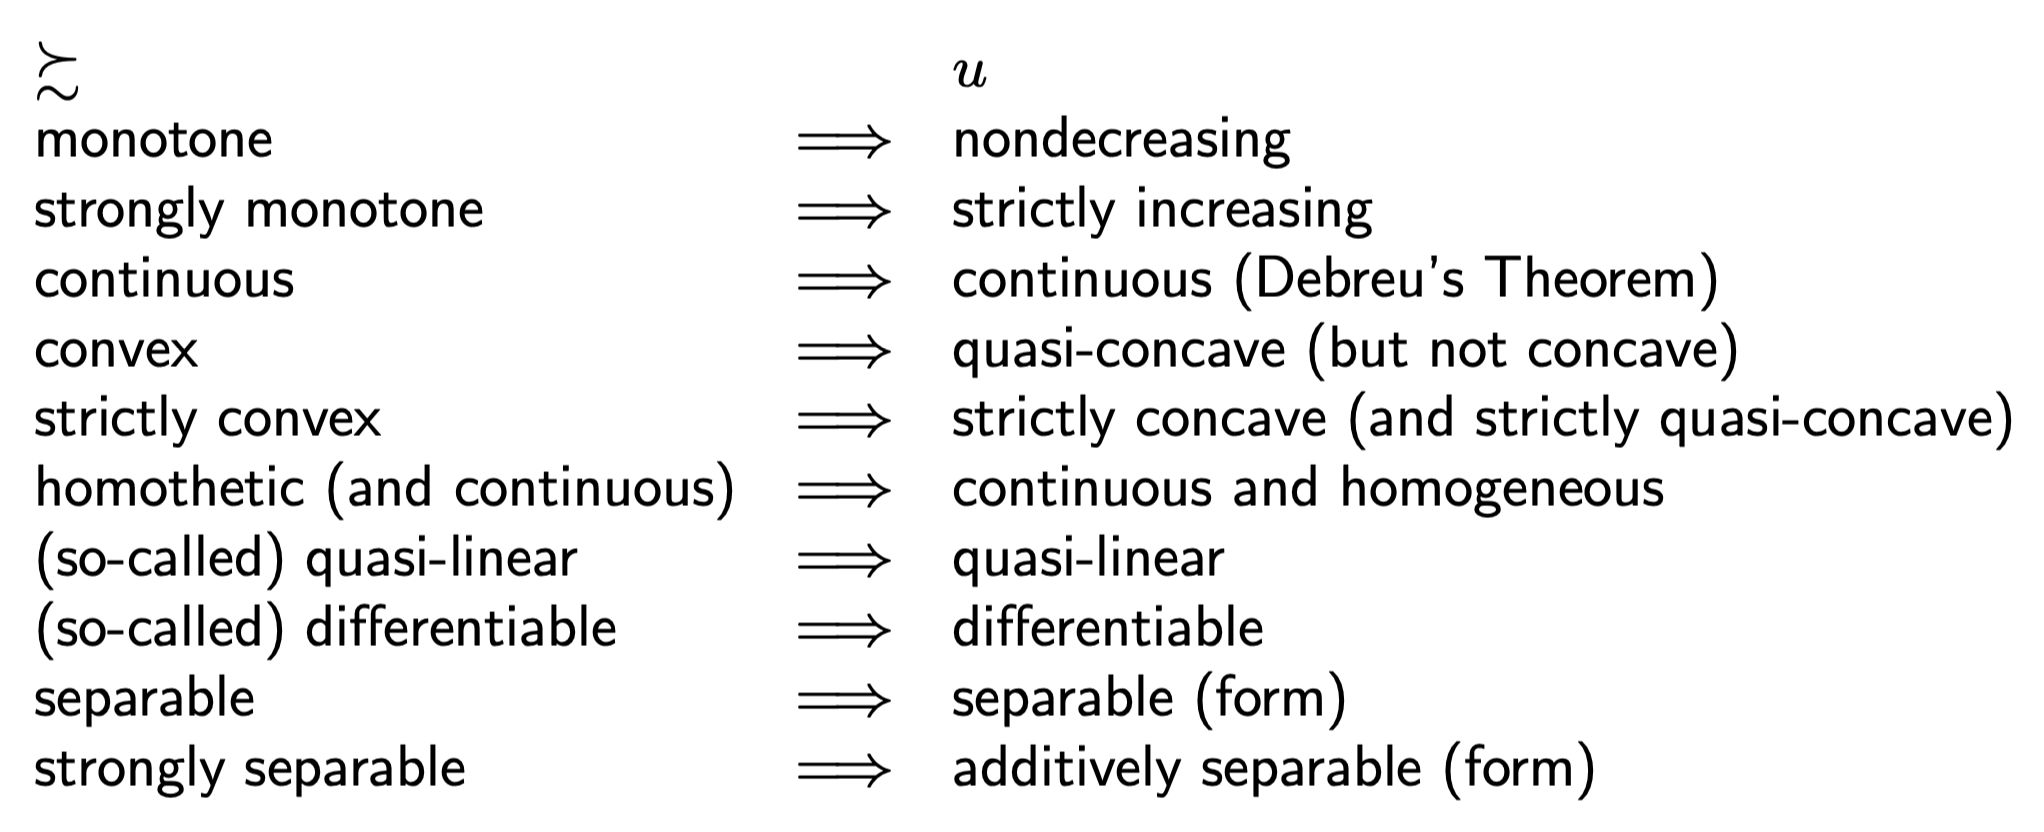
\includegraphics[scale=0.2]{Pref_prop.png}
    \caption{Properties of Preference and Utility Function}
    \label{}
\end{figure}\end{center}


\subsection{Independence of Preference}
The 'standard' model of decisions under risk is based on von Neumann and Morgenstern Expected Utility (EU), which requires the independence assumption.
\begin{definition}[Independence of Preference]
    \normalfont
    \textbf{Independence}: For any $x,y,z\in X$ and $0<\alpha<1$, if $x\succeq y$ then $\alpha x+(1-\alpha)z \succeq \alpha y+(1-\alpha)z$.
\end{definition}



\subsection{Continuous Preference}
\begin{definition}[Continuous $\succeq$]
    \normalfont
    $\succeq$ is \textbf{continuous} on $X$ \underline{if and only if} for any sequence $\{x^n,y^n\}_n=1^\infty$ with $x^n\succeq y^n$ and we note $x=\lim_{n \rightarrow \infty}x^n$, $y=\lim_{n \rightarrow \infty}y^n$, we have $x\succeq y$ (i.e., the graph $\{(x,y)\mid x\succeq y\subseteq X\times X\}$ is closed).
\end{definition}
\begin{example}[ Lexicographic preferences (not continuous)]
    Under Lexicographic preference $\succ$, $x \succ y$ \underline{if and only if}
    \begin{enumerate}[$\circ$]
        \item $x_{1}>y_{1}$, or
        \item $x_{1}=y_{1}$, and $x_{2}>y_{2}$, or
        \item $x_{1}=y_{1}$ and $x_{2}=y_{2}$ and $x_{3}>y_{3}$, or
        \item etc.
    \end{enumerate}
    Under Lexicographic preferences, there is no indifference.
    
    We can find the Lexicographic preference violates continuity: $\left(1+\frac{1}{n}, 1\right) \succ(1,2)$ and $\lim \left(1+\frac{1}{n}, 1\right)=(1,1) \prec(1,2)$.
\end{example}

\begin{proposition}[Debreu's Theorem, Continuous $\succeq$ $\Rightarrow$ continuous $u(\cdot)$]
    If $\succeq$ is continuous, then $\exists$ a continuous $u(\cdot)$ that represents $\succeq$.
\end{proposition}




\subsection{Homothetic Preference}
\begin{definition}[Homotheticity]
    \normalfont
    $\succeq$ are homothetic if $x\succeq y \Rightarrow \alpha x\succeq \alpha y$ for all $\alpha>0$.
\end{definition}

\begin{proposition}[Homothetic preference $\Leftrightarrow$ homogeneous $u(\cdot)$]
    A continuous $\succeq$ is homothetic $\Leftrightarrow$ $\exists$ a continuous homogeneous $u(\cdot)$ that represents $\succeq$ such that $u(\alpha x)=\alpha u(x)$ for all $x>0$.
\end{proposition}


\subsection{Quasi-linearity}
\begin{definition}[Quasi-Linearity]
    \normalfont
    $\succeq$ on $X$ is \textbf{quasi-linear} on $x_1$ if $$x\succeq y \Rightarrow (x+\epsilon e_1)\succeq (y+\epsilon e_1)$$ where $e_1=(1,0,...,0)$ and $\epsilon>0$.
\end{definition}

\begin{theorem}[Quasi-Linearity $\Leftrightarrow$ $u(x)=x_1+v(x_{-1})$]
    A continuous $\succeq$ on $(-\infty,\infty)\times \mathbb{R}_+^{K-1}$ is quasi-linear in $x_1$ $\Leftrightarrow$ $\exists$ a $u(\cdot)$ that represents $\succeq$ such that $$u(x)=x_1+v(x_{-1})$$
    where $v(\cdot)$ satisfies $(v(x_{-1}),0,...,0)\sim(0,x_{-1})$.
\end{theorem}

\subsection{Separability}
\begin{definition}[Separability]
    \normalfont
    $\succeq$ satisfies \textbf{separability} if for any $x_i$
    \begin{equation}
        \begin{aligned}
            (x_i, x_{-i})\succeq (x'_i, x_{-i}) \Leftrightarrow (x_i, x'_{-i})\succeq (x'_i, x'_{-i})
        \end{aligned}
        \nonumber
    \end{equation}
\end{definition}

\begin{theorem}[Separability $\Rightarrow$ Additive $u(\cdot)$]
    $\succeq$ with \textbf{separability} admits additive $u$-representation
    \begin{equation}
        \begin{aligned}
            u(x)=v_1(x_1)+\cdots v_K(x_K)
        \end{aligned}
        \nonumber
    \end{equation}
\end{theorem}

\begin{note}
    Strong assumption, usually ignored in practice.
\end{note}


\subsection{Differentiable Preference}
Consider a vector of values $v(x)\in \mathbb{R}^K_+$ for the $K$ commodities and a feasible the direction $x+\varepsilon d\in X$ from $x$ for small enough $\varepsilon>0$.

$d$ is considered \underline{improvement} if and only if $$d\cdot v(x)>0$$

Given $v(x): X \rightarrow \mathbb{R}^K_+$, let $$D_v(x)=\{d:d\cdot v(x)>0\}$$
be the set of directions that are improvements relative to $x$.

$d\in \mathbb{R}^k$ is an \underline{improvement direction} at $x$ if there is $\lambda^*>0$ such that $\lambda d$ is an improvement $$x+\lambda d\succ x$$
for any $\lambda\leq \lambda^*$. Let $D_{\succeq}(x)$ be the set of all improvement directions at $x$.

Any improvement is an improvement direction if
\begin{enumerate}[-]
    \item $\succeq$ are strictly convex.
    \item $\succeq$ are convex, strongly monotonic, and continuous.
\end{enumerate}

\begin{definition}[Differentiable Preference]
    \normalfont
    $\succeq$ is \textbf{differentiable} if there exists a function $v(x): X \rightarrow \mathbb{R}_+^K$ such that $$D_{\succeq}(x)=D_v(x),\ \forall x\in X$$
\end{definition}

\begin{example}
    $\succeq$ represented by
    \begin{enumerate}[(1).]
        \item $\alpha x_1+\beta x_2$ for $\alpha,\beta>0$ are differentiable: $v(x)=(\alpha,\beta)$.
        \item $\min\{\alpha x_1,\beta x_2\}$ are differentiable where $\alpha x_1\neq \beta x_2$: $v(x)=\left\{\begin{matrix}
            (1,0)& \textnormal{ if }\alpha x_1<\beta x_2\\
            (0,1)& \textnormal{ otherwise}
        \end{matrix}\right.$
    \end{enumerate}
\end{example}

\begin{proposition}[Sufficient condition for differentiable $\succeq$]
    Any (monotonic and convex) $\succeq$ can be represented by a (strongly monotonic and quasi-concave) and differentiable $u$ is differentiable.
\end{proposition}


\chapter{Choice Theory}
\section{Choice}
Let $\mathcal{B}=2^X$ (all subsets of $X$) and $B\in \mathcal{B}$ be the all potential alternatives that can be chosen.

The choice of an agent can be represented by $C(B)\subseteq B, \forall B\in \mathcal{B}$.
\begin{definition}[Choice Function]
    \normalfont
    A \textbf{choice function} $C$ such that $C(A)\subseteq A$ which specifies for each nonempty subset $A\subseteq X$.
\end{definition}

\begin{definition}[Induced Choice Rule]
    \normalfont
    Given a binary relation $\succeq$, the \textbf{induced choice rule} $C_\succeq$ is defined by
    $C(A)=C_\succeq(A)=\{x\in A:x\succeq y, \forall y\in A\}, \forall A\subseteq X$.\\
    A choice function $C$ can be \textbf{rationalizable} if there is a preference relation $\succeq$ on $X$ such that $C=C_\succeq$.
\end{definition}

\begin{definition}[Revealed Preference]
    \normalfont
    Given a choice rule $\succeq$, its \textbf{revealed preference relation $\succeq_C$} is defined by $x \succeq_C y$ if there exists some $A$ such that $x, y \in A$ and $x \in C(A)$.
\end{definition}

\begin{proposition}
    If $C$ is rationalized by $\succeq$, then $\succeq=\succeq_C$.
\end{proposition}

\begin{definition}[Rubinstein's Condition $\alpha$]
    \normalfont
    A choice function $C$ satisfies \textbf{condition $\alpha$} if for any two problems $A,B$, if $A\subseteq B$ and $C(B)\in A$, then $C(A)=C(B)$.
\end{definition}
%Condition $\alpha$ is sufficient for $C$ is being formulated by maximizing a preference $\succeq$.



\begin{proposition}
    Let $C$ be a choice function with a domain $D$ satisfying that if $A, B \in D$, then $A \cup B \in D$. If $C$ satisfies condition $\alpha$, then there is a preference relation $\succeq$ on $X$ such that $C = C_\succeq$.
\end{proposition}

\begin{definition}[Choice Correspondence (More than one choice)]
    \normalfont
    A choice correspondence $C$ assigns a non-empty \underline{subset} for every non-empty set $A$
    $$\emptyset\neq C(A)\subseteq A$$
\end{definition}

\begin{definition}[Sen's $\alpha$ or Independence of Irrelevant Alternatives]
    \normalfont
    If $a\in A\subseteq B$, then $a\in C(B) \Rightarrow a\in C(A)$.
\end{definition}

\begin{definition}[Sen's $\beta$]
    \normalfont
    If $a,b\in A\subseteq B$, then $a,b\in C(A)$ and $b\in c(B) \Rightarrow a\in C(B)$.
\end{definition}
$\alpha$ and $\beta$ are equivalent to WARP.


\subsection{Weak Axiom of Revealed Preference (WARP)}
\begin{definition}[Weak Axiom of Revealed Preference]\label{WARP}
    \normalfont
    Given a choice structure $(C,\mathcal{B})$ satisfies \textbf{WARP}. If $\exists B\in \mathcal{B}$ with $x,y\in B$, such that $x\in C(B)$. Then, $\forall B'\in \mathcal{B}$ with $x,y\in B'$, $y\in C(B') \Rightarrow x\in C(B')$.\\
    Or we can say, whenever $x,y\in B\cap B'$, $$x\in C(B) \textnormal{ and }y\in C(B') \Rightarrow x\in C(B')$$
\end{definition}

\begin{proposition}[Rational $\Rightarrow$ WARP]
    Given $\succeq$ is rational, then $(C^*_{\succeq},\mathcal{B})$ satisfies WARP.\\
    ($C^*_{\succeq}$ is the choice rule that picks the maximal alternatives by $\succeq$)
\end{proposition}


\section{Choice under Uncertainty}
We want to model an uncertain prospect corresponding forms of function $u$.

The literature contains (basically) three sets of answers to these questions, differing in whether uncertainty is objective or subjective.

\begin{enumerate}[$\circ$]
    \item Objective uncertainty: von Neumann-Morgenstern (vNM).
    \item Subjective uncertainty: Savage.
    \item Horse lottery-roulette wheel theory: Anscombe and Aumann (A-A)
\end{enumerate}

\subsection{von Neumann-Morgenstern (vNM)}
The set of prizes is defined by $X$ and the set of probability measures (or distributions) over $X$ is denoted by $P$.
\underline{A compound lottery:} If $p,q\in P$ and $\alpha\in[0,1]$, then there is an element $\alpha p+(1-\alpha)q\in P$ which is defined by taking the convex combinations of the probabilities of each prize separately, or
$$(\alpha p+(1-\alpha)q)(x)=\alpha p(x)+(1-\alpha)q(x)$$
$(\alpha p+(1-\alpha)q)$ represents a compound lottery.

\begin{definition}[Three Axioms]
    \normalfont
    \textbf{\underline{Three Axioms}}
    \begin{enumerate}
        \item[(A1)] $\succ$ is a preference relation (asymmetric and negatively transitive);
        \item[(A2)] For all $p,q,r\in P$ and $\alpha\in[0,1]$, $p\succ q \Rightarrow \alpha p +(1-\alpha)r\succ \alpha q+(1-\alpha)r$.
        \item[(A3)] For all $p,q,r\in P$ such that $p\succ q\succ r$, $\exists \alpha,\beta\in (0,1)$ such that
        \begin{equation}
            \begin{aligned}
                \alpha p +(1-\alpha)r\succ q\succ \beta p +(1-\beta)r
            \end{aligned}
            \nonumber
        \end{equation}
    \end{enumerate}
\end{definition}
\begin{theorem}[vNM]
    $\succ$ on $P$ satisfies axioms (A1)-(A3) if and only if there exists a function $u:X \rightarrow \mathbb{R}$ such that
    \begin{equation}
        \begin{aligned}
            p\succ q \Leftrightarrow \sum_x p(x) u(x)>\sum_x q(x) u(x)
        \end{aligned}
        \tag{*}
        \label{*}
    \end{equation}
    Moreover, $u$ is unique up to a \underline{positive affine transformation}: there is another $u'$ represents $\succ$ in the sense of (\ref{*}) if and only if there exists $c>0$ and $d$ such that
    \begin{equation}
        \begin{aligned}
            u'(\cdot)=cu(\cdot)+d
        \end{aligned}
        \nonumber
    \end{equation}
\end{theorem}
\begin{remark}
    \begin{enumerate}[$\circ$]
        \item If $u$ represents $\succ$ then so will $v(\cdot)=f(u(\cdot))$ for any \textbf{strictly increasing} $f$.
        \item $k(p)=\sum_x p(x)u(x)$ gives an ordinal representation of $\succ$.
    \end{enumerate}
\end{remark}

\begin{lemma}[Four Lemmas obtained by the three axioms]
    If $\succ$ satisfies (A1) to (A3), then
    \begin{enumerate}[(L1).]
        \item If $p\succ q$ and $0\leq\alpha<\beta\leq 1$, then $$\beta p+(1-\beta)q\succ \alpha p+(1-\alpha)q$$
        \item If $p\succeq q\succeq r$ and $p\succ r$ $\Rightarrow$ there exists a unique $\alpha^*\in[0,1]$ such that $$q\sim \alpha^*p+(1-\alpha^*)r$$
        \item If $p\sim q$ and $\alpha\in[0,1]$ $\Rightarrow$ for all $r\in P$, $$\alpha p+(1-\alpha)r\succ \alpha q+(1-\alpha)r$$
        \item For any $x\in X$, let $\delta_x$ be the probability distribution degenerate at $x$, that is $\delta_x(x')=\left\{\begin{matrix}
            1,&\textnormal{ if }x'=x\\
            0,&\textnormal{ if }x'\neq x
        \end{matrix}\right.$ For all $p\in P$, we have $x_1,x_2\in X$ such that
        \begin{equation}
            \begin{aligned}
                \delta_{x_1}\succeq p\succeq \delta_{x_2}
            \end{aligned}
            \nonumber
        \end{equation}
    \end{enumerate}
\end{lemma}

\subsection{Savage (1954)}
Consider the situation that what the decision maker chooses depends critically on his/her subjectively assesses as the odds of the outcomes.

\underline{The basics of the Savage formulation:}
\begin{enumerate}[$\circ$]
    \item a set of $X$ of prizes/consequences;
    \item a set $S$ of the nature (states of the world).
\end{enumerate}
Each $s\in S$ is a compilation of all characteristics/factors about which the DM is uncertain and which are relevant to the consequences that will
result from her/his choice. The set $S$ is an exhaustive list of mutually exclusive states — only one
$s\in S$ will be the realized state.

We denote the choice space by $H$, as the set of all functions from $S$ to $X$ ($H=X^S$).

Savage seeks to find a subjective taste (the utility function) $u(\cdot)$ and a subjective belief (the probability measure) $\pi$ such that
\begin{equation}
    \begin{aligned}
        h\succ h' \Leftrightarrow \sum_{s\in S}\pi(s)u(h(s))>\sum_{s\in S}\pi(s)u(h'(s))
    \end{aligned}
    \nonumber
\end{equation}
Note that, it contains an assumption that $u(\cdot)$ is a function about $x$ which doesn't depend on the state of the world when it receives $x$.



\section{Social Choice}
Notations:
\begin{enumerate}
    \item We consider \underline{finite} set of alternatives $X$ and \underline{finite} set of agents $I$.
    \item We use $\mathcal{B}$ to denotes the set of all preference relations.
    \item We use $\mathcal{R}\subseteq \mathcal{B}$ to denotes the set of all rational preference relations.
    \item We use $\succeq\in \mathcal{R}$ to represents individual rational preference relation.
\end{enumerate}

\subsection{Social Welfare Function and Properties}
\begin{definition}[Social Welfare Function (SWF)]
    \normalfont
    A \textbf{social welfare function} (SWF) is a mapping $$f: \mathcal{A}\subseteq \mathcal{R}^I\rightarrow \mathcal{B}$$
    $\trianglerighteq=f(\succeq_1,...,\succeq_I)$ is interpreted as the \textbf{social preference relation}. It doesn't need to be rational (i.e., complete and transitive).
\end{definition}

\begin{definition}[SWF's Properties]\label{SWF_properties}
    \normalfont
    A social welfare function $f: \mathcal{A}\rightarrow \mathcal{B}$
    \begin{enumerate}[$\circ$]
        \item has \textbf{unrestricted domain} (UD) if $\mathcal{A}=\mathcal{R}^n$;
        \item is \textbf{transitive} (T) if $f(\succeq_1,...,\succeq_I)$ is transitive for all $(\succeq_1,...,\succeq_I)\in \mathcal{A}$;
        \item is \textbf{nondictatorial} (ND) if there is no agent $i\in I$ such that $\forall \{x,y\}\subseteq X$ $x\succeq_i y \Rightarrow x\trianglerighteq y$. (That is there is no distinguished voter who can choose the winner).
        \item is \textbf{weakly Paretian} (PA) if, $\forall \{x,y\}\subseteq X$ and any preference profile $(\succeq_1,...,\succeq_I)\in \mathcal{A}$, we have $x\succeq_i y,\forall i\in I \Rightarrow x\trianglerighteq y$.
        \item is \textbf{independent of irrelevant alternatives} (IIA) if, $\forall \{x,y\}\subseteq X$, and any $\succeq$ and $\succeq'$ with $\succeq_i\mid_{x,y}=\succeq'_i\mid_{x,y}, \forall i\in I$, if $x\trianglerighteq y$ then $x\trianglerighteq' y$.
    \end{enumerate}
\end{definition}


\subsection{Arrow's Theorem}
\begin{theorem}[Arrow's impossibility theorem]
    Suppose $|X|\geq 3$, $\mathcal{A}=\mathcal{R}^I$ (UD). Then if a SWF $f$ satisfies T, PA, and IIA, then it fails to be ND.
\end{theorem}
\begin{proof}
    \normalfont
    Yu, N. N. (2012). A one-shot proof of Arrow's impossibility theorem. \textit{Economic Theory}, 523-525.
\end{proof}



\chapter{Demand Theory}
\section{Utility Maximization Problem (UMP)}
Budget set is given by $B=\{x\in X\subseteq \mathbb{R}_+^K: p\cdot x\leq w\}$, where $w$ is the DM's wealth and $p$ is the vector of prices. Without losing generality, we can assume $w=1$.

The DM's problem is finding the $\succeq$-optimal bundle $x\in B(p)$. With the corresponding utility function $u(x)$, we can consider a consumer's problem
\begin{equation}
    \begin{aligned}
        \max_{x\in X} u(x)\\
        s.t.\ p\cdot x\leq w
    \end{aligned}
    \tag{UMP}
    \label{UMP}
\end{equation}
The set $\succeq$-optimal bundle is represented by $x(p,w)$.

\subsection{Marshallian Demand: Existence and Properties}

\begin{proposition}[Continuous Preference$\Rightarrow$ Solution $x(p,w)$ Existence]
    If $\succeq$ ($u(\cdot)$) is continuous, then all such problems have a solution $x(p,w)$.
\end{proposition}
\begin{proof}
    By the Weierstrass Extreme Value Theorem.
\end{proof}

\begin{proposition}[Convex Preference$\Rightarrow$ Convex $x(p,w)$]
    If $\succeq$ is convex ($u(\cdot)$ is quasi-concave), then $x(p,w)$ is convex.
\end{proposition}
\begin{proof}
    Suppose $x,x'\in X$. The optimal utility $u^*=u(x)=u(x')$. For any $\alpha\in[0,1]$, let $x''=\alpha x+(1-\alpha)x'$. Because $\succeq$ is convex, we have $u(\cdot)$ is quasi-concave, that is $u(x'')\geq u^*$. $x''$ is also feasible. So, $x''\in x(p,w)$.
\end{proof}

\begin{proposition}[Strictly Convex Preference$\Rightarrow$ Singleton $x(p,w)$]
    If $\succeq$ is strictly convex ($u(\cdot)$ is strictly quasi-concave), then $x(p,w)$ is (at most) a singleton.
\end{proposition}

\begin{proposition}[Differentiable Preference$\Rightarrow$ Margianl Utility equals to Price]
    If $\succeq$ is differentiable, $x^*\in x(p,w)$, and the vector of marginal values at $x^*$ (as defined above) is denoted by $v(x^*)=(v_1(x^*),...,v_K(x^*))$, where $v_k(x^*)$ is usually taken by $\frac{\partial u}{\partial x_k}(x^*)$ in "classic" problem. Then, we have
    \begin{equation}
        \begin{aligned}
            \frac{v_k(x^*)}{v_j(x^*)}=\frac{p_k}{p_j} \textnormal{ for any }x^*_k,x^*_j>0
        \end{aligned}
        \nonumber
    \end{equation}
    and for any $k$ with $x_k^*>0$ (consumed commodity)
    \begin{equation}
        \begin{aligned}
            \frac{v_k(x^*)}{p_k}\geq \frac{v_j(x^*)}{p_j}\textnormal{ for any }j\neq k
        \end{aligned}
        \tag{*}
        \label{*}
    \end{equation}
\end{proposition}

\begin{corollary}[Sufficient Conditions for Optimality]
    If $\succeq$ is strongly monotonic, convex, continuous, and differentiable and if $p\cdot x^*=w$ and \eqref{*} is satisfied then $x^*\in x(p,w)$
\end{corollary}

\begin{definition}[Rationalize]
    \normalfont
    $\succeq$ \textbf{fully rationalize} the demand function $x$ if for any $(p,w)$, the bundle $x(p,w)$ is the \underline{unique} $\succeq$-maximal bundle within $B$.\\
    A monotonic $\succeq$ \textbf{rationalize} the demand function $x$ if for any $(p,w)$, the bundle $x(p,w)$ is a $\succeq$-maximal bundle within $B$.
\end{definition}

The \underline{unique} solution is called Marshallian (Uncompensated) Demand.

\begin{proposition}[Properties of Marshallian Demand]
    \begin{enumerate}[(i).]
        \item \textbf{Walras' Law}: If $\succeq$ is local nonsatiation, $\forall x^*\in x(p,w): p\cdot x^*=w$.
        \item \textbf{Homogeneity of degree zero in $( p, w )$:} $x (\alpha p, \alpha w )\equiv x ( p, w ),\ \forall \alpha > 0$.
        \item \textbf{Continuous in prices and in wealth} if the $\succeq$ is continuous.
    \end{enumerate}
\end{proposition}


\begin{proposition}[Weak Axiom of Revealed Preference of Marshallian Demand]
    If demand is single valued then WARP(\ref{WARP}) is equivalent to $$p\cdot y'\leq w \textnormal{ and }y\neq y' \Rightarrow p'\cdot y>w$$
    where $y\equiv x(p,w)$ and $y'\equiv x(p',w')$.
    ($y'$ is feasible under $(p,w)$ but $y=x(p,w)$, which means $y$ is better and it can't be feasible under $(p',w')$.)
\end{proposition}

\subsection{Lagrangian Approach: $\frac{\partial u\left(x^{*}\right)}{\partial x_{i}}=\lambda^{*} p_{i}$ and $\lambda^*\left(x_i(p,w)+\sum_{j=1}^{K} p_{j} \frac{\partial x_{j}}{\partial p_{i}}\right)=0$}
The Lagrangian of the problem is $$L(x,\lambda)=u(x)-\lambda(p \cdot x-w)$$
By the KKT necessary conditions, we have
\begin{equation}
    \begin{aligned}
        \frac{\partial L}{\partial x_{i}}(x^*,\lambda^*)=\frac{\partial u\left(x^{*}\right)}{\partial x_{i}}-\lambda^{*} p_{i}=0,\ \forall i=1,...,K\\
        \lambda^*\geq 0 \textnormal{ and } \lambda^*(p\cdot x^*-w)=0
    \end{aligned}
    \nonumber
\end{equation}
Based on that, we have
\begin{lemma}
    \begin{enumerate}[(i).]
        \item $\frac{\partial u\left(x^{*}\right)}{\partial x_{i}}=\lambda^{*} p_{i}$;
        \item $\lambda^*\left(x(p,w)+p\cdot\frac{\partial x(p,w)}{\partial p}\right)=0$ i.e., $\lambda^*\left(x_i(p,w)+\sum_{j=1}^{K} p_{j} \frac{\partial x_{j}}{\partial p_{i}}\right)=0$.
    \end{enumerate}
\end{lemma}

\subsection{Envelope Theorem $\Rightarrow \lambda^{*}=\frac{\partial u(x(p, w))}{\partial w}$}
\begin{theorem}[Envelope Theorem]
    Consider the constrained maximization problem,
    \begin{equation}
        \begin{aligned}
            \max_{x\in \mathbb{R}^n}\quad & f(x;\theta)\\
            \textnormal{s.t. }& g(x;\theta)\leq 0
        \end{aligned}
        \nonumber
    \end{equation}
    where $xin \mathbb{R}^n$ is the choice variable and $\theta\in \mathbb{R}^m$ is some parameter. Let $f,g$ be continuously differentiable real-valued functions.
    \begin{enumerate}[$\bullet$]
        \item Let the value function of the problem be $V(\theta)\triangleq f(x^*(\theta),\theta)$.
        \item The Lagrangian for this problem is $$L(x,\lambda;\theta)=f(x; \theta)-\lambda g(x; \theta)$$
        \item Let $x^{*}$ and $\lambda^{*}$ denote the optimized values of the variables.
        \item[](By KKT necessary conditions, we have $\frac{\partial f}{\partial x}(x^*;\theta)=\lambda^* \frac{\partial g}{\partial x}(x^*;\theta)$ and $\lambda^* g(x^*;\theta)=0$)
    \end{enumerate}
    Then the following is true for any $\bar{\theta}\in \mathbb{R}^m$
    \begin{equation}
        \begin{aligned}
            \frac{\partial V}{\partial \theta_i}(\bar{\theta})=\frac{\partial L}{\partial \theta_i}(x^{*}, \lambda^{*};\bar{\theta})=\frac{\partial f}{\partial \theta_i}(x^{*};\bar{\theta})-\lambda^*\frac{\partial g}{\partial \theta_i}(x^{*};\bar{\theta})
        \end{aligned}
        \nonumber
    \end{equation}
\end{theorem}
\begin{proof}
    The proof of the envelope theorem is a straightforward calculation.\\
    Firstly, by KKT necessary conditions, we have $\frac{\partial f}{\partial x}(x^*;\bar{\theta})=\lambda^* \frac{\partial g}{\partial x}(x^*;\bar{\theta})$ and $\lambda^* g(x^*;\bar{\theta})=0 \Rightarrow \lambda^*\left[\frac{\partial g}{\partial x}(x^*;\bar{\theta})\frac{\partial x^*(\bar{\theta})}{\partial \theta_i}+\frac{\partial g}{\partial \theta_i}(x^*;\bar{\theta})\right]=0$. Then we have
    \begin{equation}
        \begin{aligned}
            \frac{\partial V}{\partial \theta_i}(\bar{\theta})&=\frac{\partial f}{\partial \theta_i}(x^*;\bar{\theta})+\frac{\partial f}{\partial x}(x^*;\bar{\theta})\frac{\partial x^*(\bar{\theta})}{\partial \theta_i}\\
            &\left(\textnormal{by }\frac{\partial f}{\partial x}(x^*;\bar{\theta})=\lambda^* \frac{\partial g}{\partial x}(x^*;\bar{\theta})\right)\\
            &=\frac{\partial f}{\partial \theta_i}(x^*;\bar{\theta})+\lambda^* \frac{\partial g}{\partial x}(x^*;\bar{\theta})\frac{\partial x^*(\bar{\theta})}{\partial \theta_i}\\
            &\left(\textnormal{by }\lambda^*\left[\frac{\partial g}{\partial x}(x^*;\bar{\theta})\frac{\partial x^*(\bar{\theta})}{\partial \theta_i}+\frac{\partial g}{\partial \theta_i}(x^*;\bar{\theta})\right]=0\right)\\
            &=\frac{\partial f}{\partial \theta_i}(x^{*};\bar{\theta})-\lambda^*\frac{\partial g}{\partial \theta_i}(x^{*};\bar{\theta})
        \end{aligned}
        \nonumber
    \end{equation}
\end{proof}

\begin{corollary}\label{corollary:marginal_wealth}
    $\lambda^{*}=\frac{\partial u(x(p, w))}{\partial w}$.
\end{corollary}
\begin{proof}
    By the envelope theorem, we have $\frac{\partial u(x(p, w))}{\partial w}=\left.\frac{\partial L}{\partial w}\right|_{x^{*}, \lambda^{*}}=\lambda^{*}$.
\end{proof}

\subsection{Indirect Utility Function $v(p, w) \equiv u(x(p, w))$}
\begin{proposition}[Properties of Indirect Utility Function]
    \begin{enumerate}
        \item $v(p,w)$ is homogeneous of degree zero in $(p, w)$;
        \item $v(p,w)$ is strictly increasing in $w$ and non-increasing in $p_{i}$;
        \item $v(p,w)$ is quasi-convex, that is the set $\{p:v(p,w)\leq u\}$ is convex for all $u\in \mathbb{R}$.
        \item $\lambda^{*}=\frac{\partial v(p, w)}{\partial w}$ (Corollary \ref{corollary:marginal_wealth}).
    \end{enumerate}
\end{proposition}

\subsection{Roy's Identity $x^*_i=-\frac{\frac{\partial v}{\partial p_{i}}}{\frac{\partial v}{\partial w}}$: recover $x(p, w)$ from $v(p, w)$}
\begin{proposition}[Roy's Identity]
    $x^*_i(p,w)=-\frac{\frac{\partial v(p,w)}{\partial p_{i}}}{\frac{\partial v(p,w)}{\partial w}}$.
\end{proposition}
\begin{proof}
    By the definition,
    \begin{equation}
        \begin{aligned}
            v(p, w) & \equiv u(x(p, w))&\\
            \frac{\partial v}{\partial p_{i}} & \equiv \sum_{j=1}^{K} \frac{\partial u}{\partial x_{j}} \frac{\partial x_{j}}{\partial p_{i}}&\\
            &=\sum_{j=1}^{K} \lambda^{*} p_{j} \frac{\partial x_{j}}{\partial p_{i}}& \textnormal{ by }\frac{\partial u\left(x^{*}\right)}{\partial x_{i}}=\lambda^{*} p_{i}\\
            &=-\lambda^{*} x_{i}^{*}&\textnormal{ by }\lambda^*\left(x_i(p,w)+\sum_{j=1}^{K} p_{j} \frac{\partial x_{j}}{\partial p_{i}}\right)=0\\
            x^*_i&=-\frac{\frac{\partial v}{\partial p_{i}}}{\frac{\partial v}{\partial w}}&\textnormal{ by }\lambda^{*}=\frac{\partial v(p, w)}{\partial w}
        \end{aligned}
        \nonumber
    \end{equation}
\end{proof}

\section{Expenditure Minimization Problem (EMP)}
Consider the duality
\begin{equation}
    \begin{aligned}
        \min_{x\in X}\quad & p\cdot x\\
        s.t.\quad & u(x)\geq u
    \end{aligned}
    \tag{EMP}
    \label{EMP}
\end{equation}
The optimal solutions are represented by $h(p,u)$. With uniqueness, we call it \textit{Hicksian (compensated) demand}.

\subsection{Hicksian Demand $h(p,u)$: Properties}
\begin{proposition}[Properties of Hicksian Demand]
    \begin{enumerate}[(i).]
        \item $h(p,u)$ is homogeneous of degree zero in $p$: $$h(tp,u)=h(p,u),\ \forall t\in \mathbb{R}_+$$
        \item $u ( x )$ is strictly quasi-concave $\Rightarrow$ $h ( p, u )$ is unique;
        \item For $u>u(0)$ and $u(\cdot)$ is locally non-satiated, \underline{constraint is active}: for all $x^*\in h(p,u)$, $$u(x^*)=u$$
    \end{enumerate}
\end{proposition}

\begin{lemma}[$\sum_{j=1}^{K} \frac{\partial u}{\partial x_j} \frac{\partial h_{j}}{\partial p_{i}}=0$]
    If $u ( x )$ is strictly quasi-concave, the Hicksian demand satisfies $\sum_{j=1}^{K} \frac{\partial u}{\partial x_j} \frac{\partial h_{j}}{\partial p_{i}}=0$
\end{lemma}
\begin{proof}
    $u(h(p,u))\equiv u \Rightarrow \sum_{j=1}^{K} \frac{\partial u}{\partial x_j}\frac{\partial h_{j}}{\partial p_{i}}=0$.
\end{proof}

\subsection{Expenditure Function $e(p,u)\equiv p\cdot h(p,u)$}
Given the Hicksian demand $h(p,u)$, we can define the expenditure function as $e(p,u)\equiv p\cdot h(p,u)$.
\begin{proposition}[Properties of Expenditure Function]\label{expen}
    \begin{enumerate}[(i).]
        \item $e ( p, u )$ is homogeneous of degree $1$ in $p$: $$e(tp,u)=tp\cdot h(tp,u)=tp\cdot h(p,u)=t e(p,u)$$
        \item $e ( p, u )$ is strictly increasing in $u$, non-decreasing in $p_i$;
        \item $e ( p, u )$ is \textbf{concave} in $p$;
        \item $e ( p, u )$ is continuous in $p$ for all $p>>0$;
        \item For all $x^*\in h(p,u)$, $x^*\in x(p,e(p,u))$;
        \item For $w>0$, $e(p,v(p,w))\equiv w$;
        \item $e(p,u)$'s derivative property: $$\frac{\partial e(p, u)}{\partial p_{i}} \equiv h_{i}(p, u)$$
    \end{enumerate}
\end{proposition}
\begin{proof}[Proof for concavity]
    Suppose the price of good 1 increases from $p_1^0$ to $p_1^1$: $p^0 \rightarrow	p^1$. Set $p^a=ap^0+(1-a)p^1,\ 0\leq a\leq 1$. So, $p^0\leq p^a\leq p^1$ and
    \begin{equation}
        \begin{aligned}
            e(p^a,u)&=p^a\cdot h(p^a,u)\\
            &=(ap^0+(1-a)p^1)\cdot h(p^a,u)\\
            &=a[p^0\cdot h(p^a,u)]+(1-a)[p^1\cdot h(p^a,u)]\\
            &h(p^a,u)\text{ is feasible in both EMP, but not optimal solutions}\\
            &\geq a[p^0\cdot h(p^0,u)]+(1-a)[p^1\cdot h(p^1,u)]\\
            &= ae(p^0,u)+(1-a)e(p^1,u)
        \end{aligned}
        \nonumber
    \end{equation}
\end{proof}

\begin{proof}[Proof for Derivative]
    \begin{enumerate}
        \item \underline{Direct proof:}
        $$
        \begin{aligned}
        e(p, u) & \equiv p \cdot h(p, u)& \\
        \frac{\partial e}{\partial p_{i}} & \equiv \sum_{j=1}^{K} p_{j} \frac{\partial h_{j}}{\partial p_{i}}+h_{i}& \\
        & \equiv \sum_{j=1}^{K} \frac{1}{\lambda^{*}} \frac{\partial u\left(x^{*}\right)}{\partial x_{j}} \frac{\partial h_{j}}{\partial p_{i}}+h_{i}& \textnormal{ by }\frac{\partial u\left(x^{*}\right)}{\partial x_{i}}=\lambda^{*} p_{i}\\
        &=h_i&\textnormal{ by }\sum_{j=1}^{K} \frac{\partial u}{\partial x_j} \frac{\partial h_{j}}{\partial p_{i}}=0
        \end{aligned}
        $$
        \item \underline{Envelope Theorem Proof:}
        \begin{equation}
            \begin{aligned}
                L(x,\lambda;(p,u))&=p\cdot x-\lambda (u(x)-u)\\
                \frac{\partial e(p,u)}{\partial p_i}&=\frac{\partial L(x,\lambda;(p,u))}{\partial p_i}\bigg|_{x^*=h(p,u)}=x_i|_{x^*=h(p,u)}=h_i(p,u)
            \end{aligned}
            \nonumber
        \end{equation}
    \end{enumerate}
\end{proof}

\subsection{Law of Compensated Demand: $\frac{\partial h_i}{\partial p_i}\leq 0$}
\begin{corollary}[Law of Compensated Demand]
    Hicksian demand is downward sloping in its own price, $$\frac{\partial h_i}{\partial p_i}\leq 0$$
\end{corollary}
\begin{proof}
    By the concavity of $e(p,u)$ (\ref{expen}), we can conclude $\nabla^2 e(p,u)\preceq 0$ (negative semi-definite). Then, we know its diagonal elements are non-positive $\frac{\partial e^2}{\partial^2 p_i}=\frac{\partial h_i}{\partial p_i}\leq 0$.
\end{proof}

\subsection{Shifts in Hicksian Demand: $\frac{\partial h_{i}}{\partial u}  \equiv \frac{\partial x_{i}}{\partial w} \frac{\partial e}{\partial u}$, same direction as $\frac{\partial x_{i}}{\partial w}$}
How does Hicksian demand curve shift when utility changes?
$$
\begin{aligned}
h_{i}(p, u) & \equiv x_{i}(p, e(p, u)) \\
\frac{\partial h_{i}}{\partial u} & \equiv \frac{\partial x_{i}}{\partial w} \frac{\partial e}{\partial u}
\end{aligned}
$$
We know $\frac{\partial e}{\partial u}>0$, so the direction of Hicksian demand shift is the same as $\frac{\partial x_{i}}{\partial w}$.\\
- Normal good: increasing utility shifts $h_{i}$ to the right.\\
- Inferior good: increasing utility shifts $h_{i}$ to the left.

\section{UMP and EMP}
\subsection{Slutsky Equation: substitution effect and income effect}
Slutsky: how change of $p_j$ (price in good $j$) affects $x_i$ (the demand of product $i$).
\begin{proposition}[Slutsky Equation]
    \begin{equation}
        \begin{aligned}
            \frac{\partial x_i(p,w)}{\partial p_j}=\underbrace{\frac{\partial h_i(p,u)}{\partial p_j}}_{\textnormal{substitution effect}}\underbrace{-\frac{\partial x_i(p,w)}{\partial w} x_j(p,w)}_{\textnormal{income effect}}
        \end{aligned}
        \nonumber
    \end{equation}
\end{proposition}
\begin{proof}
    \begin{equation}
        \begin{aligned}
            h_i(p,u)&\equiv x_i(p,e(p,u))\\
            \frac{\partial h_{i}}{\partial p_{j}} & \equiv \frac{\partial x_{i}}{\partial p_{j}}+\frac{\partial x_{i}}{\partial w} \frac{\partial e}{\partial p_{j}} \\
            & \equiv \frac{\partial x_{i}}{\partial p_{j}}+\frac{\partial x_{i}}{\partial w} h_{j}(p, u) \\
            & \equiv \frac{\partial x_{i}}{\partial p_{j}}+\frac{\partial x_{i}}{\partial w} x_{j}(p, e(p,u))
        \end{aligned}
        \nonumber
    \end{equation}
\end{proof}
\begin{enumerate}[$\circ$]
    \item \textbf{Substitution effect}: $\frac{\partial h_{i}}{\partial p_{j}}$, the change of relative prices change with constant utility will change the $x_i$.
    \item \textbf{Income (Wealth) effect}: $-\frac{\partial x_{i}}{\partial w} x_{j}(p, w)$, the change of price can be seen as change of wealth, which will also impact the $x_i$.
\end{enumerate}

\subsection{Relationship Between UMP and EMP}
\begin{center}\begin{figure}[htbp]
    \centering
    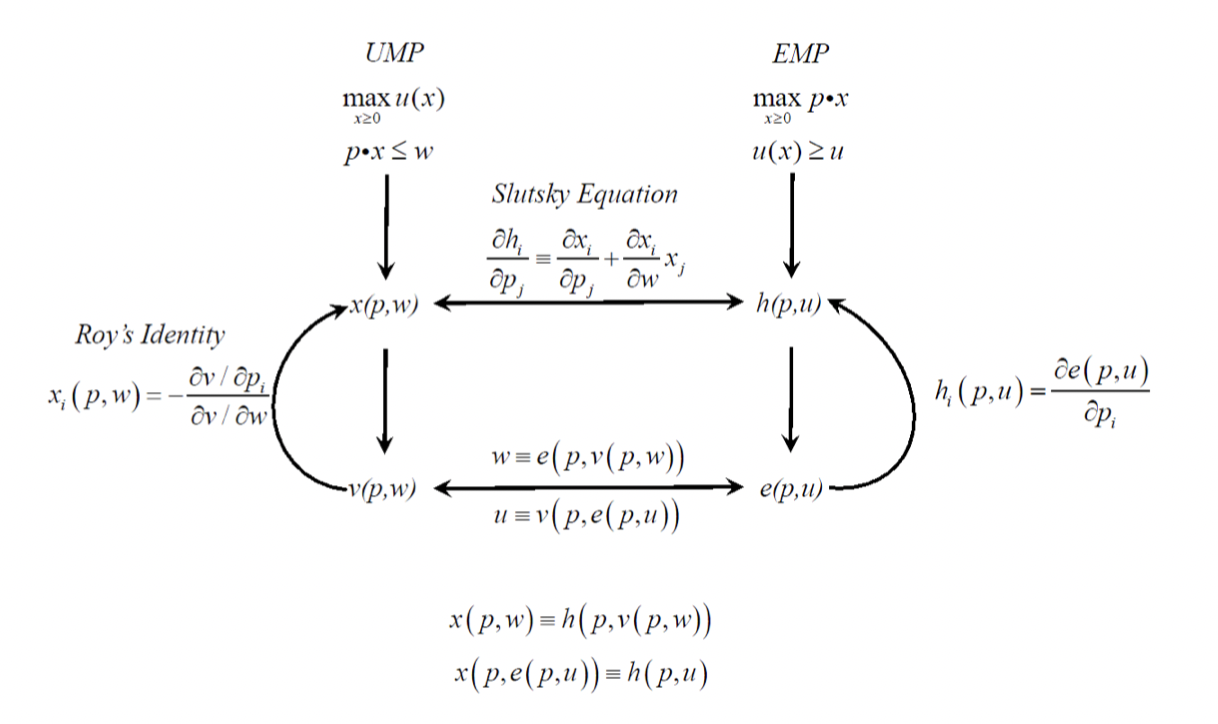
\includegraphics[scale=0.6]{UMP-EMP.png}
    \caption{Relationship Between UMP and EMP}
    \label{}
\end{figure}\end{center}


\section{Competitive Equilibrium}
\begin{definition}[Competitive Equilibrium]
    \normalfont
    Given endowment $\{w^i\}_{i\in I}$. A \textbf{competitive equilibrium} is a pair $p\in \mathbb{R}^L$ (price vector over $L$ goods) and an allocation $(x^i)_{i\in I}$ such that:
    \begin{enumerate}[(i).]
        \item $x^i\in \argmax u^i(x)$ s.t. $p\cdot x^i\leq p\cdot w^i, \forall i\in I$.
        \item $\sum_{i\in I}x^i_\rho (p,w)=\sum_{i\in I}w^i_\rho, \forall \rho\in L$.
    \end{enumerate}
\end{definition}

\begin{definition}
    \normalfont
    An allocation $x$ is \textbf{Pareto-effecient} if there doesn't exist an allocation $y$ s.t. $u_i(y)\geq u_i(x)$ for each $i\in I$ and $u_j(y)> u_j(x)$ for some $j\in I$.
\end{definition}

(Assume consumers' preferences are strict monotone)
\begin{theorem}[First-order fundamental welfare theorem]
    Suppose $(p^*,x^*)$ is a competitive equilibrium. Then $x^*$ is Pareto-efficient.
\end{theorem}

If CE exists we can prove a Pareto-effecient allocation is CE.
\begin{theorem}[Second-order fundamental welfare theorem]
    Suppose that $x^*$ is Pareto efficient and consumers receive endowment worth $w^i=p\cdot {x^i}^*$ for all $i\in I$. Then, if a competitive equilibrium exists for such $w$, then $x^*$ is a competitive equilibrium allocation.
\end{theorem}







\chapter{Game Theory}
Based on
\begin{enumerate}[$\circ$]
    \item "Kreps, D. M., \& Sobel, J. (1994). Signalling. \textit{Handbook of game theory with economic applications}, 2, 849-867."
    \item Mas-Colell, Whinston, and Green, Microeconomic Theory, Oxford University Press (1995).
    \item UIUC ECON 530 21Fall, Nolan H. Miller
    \item UC Berkeley ECON 201A 23Fall
    \item UC Berkeley MATH 272 23Fall, Alexander Teytelboym
    \item  Jehle, G., Reny, P.: Advanced Microeconomic Theory . Pearson, 3rd ed. (2011). Ch. 6.
\end{enumerate}



\section{Basic Game Theory}

\subsection{Game, Dominant Strategy}
A game is denoted by $$\Gamma =\left(\underbrace{I}_{\textnormal{players}},\underbrace{\{S_i\}_{i\in I}}_{\textnormal{Strategy Set}},\underbrace{\{u_i(\cdot)\}_{i\in I}}_{\textnormal{VNM utility}}\right)$$

$u_i:\prod_{i\in I}S_i \rightarrow \mathbb{R}$ is the utility function that maps all players' strategies to a player's utilities.

\begin{definition}[Dominant Strategy]
    \normalfont
    A strategy $s_i\in S_i$ is \textbf{dominant} for $i$ in $\Gamma$ if for all $s'_i\neq s_i$, we have $u_i(s_i,S_{-i})\geq u_i(s'_i,S_{-i})$.
\end{definition}

\subsection{Nash Equilibrium and Existence}
\begin{definition}[Nash Equilibrium]
    \normalfont
    A strategy profile $\Sigma=(\sigma_1,...,\sigma_I)$ is a \textbf{Nash} equilibrium of the game $\Gamma$ if for every $i\in I$, we have: $u_i(\sigma^*_i,\sigma^*_{-i})\geq u_i(\sigma'_i,\sigma^*_{-i}), \forall \sigma'_i\in \Delta(S_i)$ (can't benefit from deviating).
\end{definition}

\begin{theorem}[Existence of Nash Equilibrium]
    A Nash equilibrium exists in $\Gamma$ if for all $i\in I$,
    \begin{enumerate}[(i).]
        \item $S_i$ is non-empty, convex, compact, subset of $\mathbb{R}^m$ (i.e., for some finite dimensions of real numbers).
        \item $u_i(s_i,...,s_I)$ is continuous in $(s_i,...,s_I)$ and quasi-concave in any $s_i$.
    \end{enumerate}
\end{theorem}
\begin{proof}
    We prove a lemma for the best response correspondence $b_i(s_{-i})=\argmax_{s_i\in S_i}u(s_i,s_{-i})$ firstly.
    \begin{lemma}
        Suppose $\{S_i\}_{i\in I}$ are non-empty. Suppose that $S_i$ is compact and convex and $u_i$ is continuous in $(s_i,...,s_I)$ and quasi-concave in any $s_i$, then $b_i(s_{-i})$ is non-empty, convex-valued and uhc.
    \end{lemma}
    \begin{proof}
        This lemma is proved by Berge's Maximum Theorem (Theroem \ref{thm:Berge's Maximum Theorem}).
    \end{proof}
    Consider the function $b: S \rightarrow S$ with $b(s_i,...,s_I)=\{b_1(s_{-1}),...,b_I(s_{-I})\}$.

    As we proved $b$ is non-empty, convex-valued and uhc from $S$ to $S$ where $S$ is non-empty, compact, and convex. By the Kakutani's Fixed Point Theorem (Theorem \ref{thm:Kakutani's Fixed Point Theorem}), we have $b$ has a fixed point $s\in S$, which should be the Nash equilibrium.
\end{proof}

\subsection{Bayesian Game}
\begin{definition}[Bayesian Game]
    \normalfont
    A \textbf{Bayesian game} is defined by $\Gamma=(I, \{S_i\}_{i\in I}, \{u_i(\cdot)\}_{i\in I},\{\Theta_i\}_{i\in I}, \{F_i\}_{i\in I})$
    where $u_i(s_i,s_{-i},\theta_i)$ maps the strategies of players and player $i$'s type $\theta_i\in \Theta_i$ to player $i$'s utilities. $F_i$ is the distribution of the player $i$'s type.
\end{definition}


\section{Mechanism Design}
Design incentives for agents to reveal their types or achieve particular society outcomes.

Given the set of agents, alternatives (for the society), and types (of agents) are $I, X, \Theta$ and a social choice function $f:\Theta=(\Theta_1,...,\Theta_I) \rightarrow X$.

\begin{definition}[Mechanism]
    \normalfont
    A \textbf{mechanism} is represented as $$\Gamma=\left((S_1,...,S_I), g:S\triangleq(S_1,...,S_I) \rightarrow X\right)$$
    where $S_i$ represents the strategy set of agent $i$.
\end{definition}

\begin{definition}[Implement]
    \normalfont
    $\Gamma$ (indirectly) \textbf{implements} a social choice function $f$ if $\exists \left(s_1^*(\cdot),...,s_I^*(\cdot)\right)$ of a game induced by $\Gamma$ such that $g(s_1^*(\theta_1),...,s_I^*(\theta_I))=f(\theta_1,...,\theta_I)$ for all $(\theta_1,...,\theta_I)\in \Theta$
\end{definition}

\begin{definition}[Direct Mechanism]
    \normalfont
    A mechanism is \textbf{direct mechanism} if $S_i=\Theta_i$ for all $i\in I$ and $g(\theta)=f(\theta)$ for all $\theta=(\theta_1,...,\theta_I)\in\Theta$. So, a direct mechanism can be represented by $\Gamma=(\Theta,f(\cdot))$.
\end{definition}

\begin{definition}[Weak Dominance]
    \normalfont
    A strategy is weakly dominant if for all $\theta_i\in\Theta_i$ and all $s_{-i}(\cdot)\in S_{-i}$, we have:
    $$u_i(g(s_i(\theta_i),s_{-i}),\theta_i)\geq u_i(g(s'_i,s_{-i}),\theta_i)$$
    for all $s'_i\neq s_i$.
\end{definition}

\begin{definition}[Dominant Strategy Equilibrium]
    \normalfont
    Strategy profile $s^*=(s_1^*(\cdot),...,s_I^*(\cdot))$ is a \textbf{dominant strategy (D-S) equilibrium} of $\Gamma=(S,g(\cdot))$ if for all $i\in I$ and $\theta_i\in \Theta$, we have:
    \begin{equation}
        \begin{aligned}
            u_i(g(s_i^*(\theta_i),s_{-i}),\theta_i)&\geq u_i(g(s'_i,s_{-i}),\theta_i)
        \end{aligned}
        \nonumber
    \end{equation}
    for all $s'_i\in S_i$ and $s_{-i}\in S_{-i}$.
\end{definition}

\begin{definition}[Implement in dominant strategies]
    \normalfont
    $\Gamma$ \textbf{implements} $f$ in \textbf{dominant strategies} if $\exists$ a dominant strategy (D-S) equilibrium $s^*$ of $\Gamma$ such that $g(s^*(\theta))=f(\theta)$.
\end{definition}

\begin{definition}[Strategy-Proof, DSIC]
    \normalfont
    $f$ is \textbf{strategy-proof} (also called dominant-strategy-incentive-compatible, DSIC) if "$s^*_i(\theta_i)=\theta_i$ for all $\theta_i\in\Theta_i$ and all $i\in I$" is a dominant strategy (D-S) equilibrium of the direct mechanism $\Gamma=(\Theta,f(\cdot))$.
\end{definition}

\begin{theorem}[Revelation Principle]
    Suppose that $\exists \Gamma=(S,g(\cdot))$ that (indirectly) implements $f$ in dominant strategies. Then $f$ is strategy-proof (DSIC).
\end{theorem}

\begin{center}\begin{figure}[htbp]
    \centering
    \begin{tikzpicture}[domain=0:3.25]
        \node at (0,0) {Types: $\Theta$};
        \draw[->](1,0)--(7,0) node[right] {Alternatives: $X$};
        \draw[dashed,->](0.5,-0.5)--(3.5,-3);
        \node at (4,-3) {$s^*(\theta)$};
        \draw[dashed,->](4.5,-3)--(7.5,-0.5);
        \draw[->](0,-0.5)--(3.5,-3.5);
        \node at (4,-3.5) {$s^*=\theta$};
        \draw[->](4.6,-3.5)--(8.1,-0.5);
        \node at (0.5,-1.8) {Desirable};
        \node at (0.5,-2.2) {Situation};
        \node at (2.5,-1.3) {Mechanism};
        \node at (2.5,-1.7) {$\Gamma$};
        \node at (6.5,-2.5) {$f(\theta)$};
        \node at (5.5,-1.5) {$g(s^*(\theta))$};
    \end{tikzpicture}
    \caption{How Mechanism Design works}
    \label{}
\end{figure}\end{center}

\begin{theorem}[Gibbard-Satterthwaite theorem]
    Suppose that $|X|\geq 3$ and a social choice function $f$ is surjective. Then,
    \begin{center}
        $f$ is strategy-proof (DSIC) $\Leftrightarrow$ $f$ is dictatorial (\ref{SWF_properties})
    \end{center}
\end{theorem}
Some lemmas can help to prove the theorem.
\begin{lemma}
    If $f$ is strategy-proof (DSIC) and $f(\succeq)=x$ and $x\succeq_i y \Rightarrow x\succeq'_i y$ for all $i\in I$ and all $x\neq y\in X$, then $f(\succeq')=x$.
\end{lemma}

\begin{lemma}[Pareto Effeciency]
    If $f$ is strategy-proof (DSIC) and $x\succ_i y$ for all $i\in I$, then $f(\succeq')\neq y$.
\end{lemma}

\begin{example}
    Define $\succeq=\begin{pmatrix}
        x&y\\
        y&x\\
        z&z
    \end{pmatrix}$ and $\succeq'=\begin{pmatrix}
        x&y\\
        y&z\\
        z&x
    \end{pmatrix}$, each column 1/2 represents player 1/2's preferences.
\end{example}






\section{Signaling Game}
\subsection{Canonical Game}
\begin{definition}[Canonical Game]
    \normalfont
    \begin{enumerate}
        \item There are two players: $\mathbf{S}$ (sender) and $\mathbf{R}$ (receiver).
        \item $\mathbf{S}$ holds more information than $\mathbf{R}$: the value of some random variable $t$ with support $\mathcal{T}$. (We say that $t$ is the \textbf{type} of $\mathbf{S}$)
        \item Prior belief of $\mathbf{R}$ concerning $t$ are given by a probability distribution $\rho$ over $\mathcal{T}$ (common knowledge)
        \item $\mathbf{S}$ sends a \textbf{signal $s\in \mathcal{S}$} to $\mathbf{R}$ drawn from a signal set $\mathcal{S}$.
        \item $\mathbf{R}$ receives this signal, and then takes an \textbf{action} $a\in \mathcal{A}$ drawn from a set $\mathcal{A}$ (which could depend on the signal $s$ that is sent).
        \item $\mathbf{S}$'s payoff is given by a function $u: \mathcal{T}\times \mathcal{S} \times \mathcal{A} \rightarrow \mathbb{R}$ and $\mathbf{R}$'s payoff is given by a function $v: \mathcal{T}\times \mathcal{S} \times \mathcal{A} \rightarrow \mathbb{R}$.
    \end{enumerate}
\end{definition}

\subsection{Nash Equilibrium}
\begin{definition}[Strategy]
    \normalfont
    A \textbf{behavior strategy} for $\mathbf{S}$ is given by a function $\sigma: \mathcal{T}\times\mathcal{S} \rightarrow [0,1]$ such that $\sum_s \sigma(t,s)$ for each $t$.\\
    A \textbf{behavior strategy} for $\mathbf{R}$ is given by a function $\alpha: \mathcal{S}\times\mathcal{A} \rightarrow [0,1]$ such that $\sum_a \alpha(s,a)$ for each $t$.
\end{definition}

\begin{definition}[Nash Equilibrium]
    \normalfont
    Behavior strategies $\alpha$ and $\sigma$ form a \textbf{Nash equilibrium} if and only if
    \begin{enumerate}
        \item For all $t\in \mathcal{T}$,
        \begin{center}
            $\sigma(t,s)>0$ implies $\sum_a \alpha(s,a)u(t,s,a) = \max_{s'\in \mathcal{S}}\left(\sum_a \alpha(s',a)u(t,s',a)\right)$
        \end{center}
        \item For each $s\in \mathcal{S}$ such that $\sum_{t}\sigma(t,s)\rho(t)>0$,
        \begin{center}
            $\alpha(s,a)>0$ implies $\sum_{t}\mu(t;s)v(t,s,a) = \max_{a'}\sum_{t}\mu(t;s)v(t,s,a')$
        \end{center}
        where $\mu(t;s)$ is the $\mathbb{R}$'s posterior belief about $t$ given $s$, $\mu(t;s)=\frac{\sigma(t,s)\rho(t)}{\sum_{t'}\sigma(t',s)\rho(t')}$ if $\sum_t\sigma(t,s)\rho(t)>0$ and $\mu(t;s)=0$ otherwise.
    \end{enumerate}
\end{definition}

\begin{definition}[Separating \& Pooling Equilibrium]
    \normalfont
    An equilibrium $(\sigma,\alpha)$ is called a \textbf{separating} equilibrium if each type $t$ sends different signals; i.e., the set $\mathcal{S}$ can be partitioned into (disjoint) sets $\{\mathcal{S}_t; t\in \mathcal{S}\}$ such that $\sigma(t, \mathcal{S}_t) = 1$. An equilibrium $(\sigma,\alpha)$ is called a \textbf{pooling} equilibrium if there is a single signal $s^*$ that is sent by all types; i.e., $\sigma(t, s^*) = 1$ for all $t\in \mathcal{T}$.
\end{definition}


\subsection{Single-crossing}

\subsubsection{Situation over real line}
Consider the situation that $\mathcal{T},\mathcal{S},\mathcal{A}\subseteq \mathbb{R}$ and $\geq$ is the usual "greater than or equal to" relationship.

\begin{enumerate}
    \item We let $\Delta \mathcal{A}$ denote the set of probability distributions on $\mathcal{A}$.
    \item For each $s\in \mathcal{S}$ and $\mathcal{T}'\subseteq \mathcal{T}$, we let $\Delta\mathcal{A}(s,T')$ be the set of mixed strategies that are the best responses by $\mathbf{R}$ to $s\in \mathcal{S}$ for some probability distribution with support $\mathcal{T}'$.
    \item For $\alpha\in \Delta\mathcal{A}$, we write $u(t,s,\alpha)\triangleq \sum_{a\in \mathcal{A}}u(t,s,a)\alpha(a)$.
\end{enumerate}

\begin{definition}[Single-crossing]
    \normalfont
    The data of the game are said to satisfy the \textbf{single-crossing property} if the following holds: If $t\in \mathcal{T}$, $(s,\alpha)\in \mathcal{S}\times \Delta\mathcal{A}$ and $(s',\alpha')\in \mathcal{S}\times \Delta\mathcal{A}$ are such that $\alpha\in \Delta\mathcal{A}(s,\mathcal{T})$, $\alpha'\in \Delta\mathcal{A}(s',\mathcal{T})$, $s>s'$ and $u(t,s,\alpha)\geq u(t,s',\alpha')$, then for all $t'\in T$ such that $t'>t$, $u(t',s,\alpha)\geq u(t',s',\alpha')$.
\end{definition}



\section{Equilibrium Refinement}
\subsection{Cho-Kreps Intuitive Criterion}
\begin{definition}[Equilibrium Dominated Message]
    \normalfont
    A message is \textbf{equilibrium dominated} for a type if the type must do strictly worse by sending the message than it does in equilibrium (i.e., payoff in eq. is strictly better than maximum payoff from deviating).
\end{definition}

\begin{definition}[Cho-Kreps Intuitive Criterion]
    \normalfont
    If an information set is off the eq. path and a message is eq. dominated for a type, then beliefs should assign zero probability to the message coming from that type (if possible).
\end{definition}















\chapter{Market Design}
Based on
\begin{enumerate}[$\circ$]
    \item Two-Sided Matching: A Study in Game-Theoretic Modeling and Analysis, Roth, Alvin E.\& Sotomayor, Matilda, 1990.
    \item Fleiner, T. (2003). A fixed-point approach to stable matchings and some applications. \textit{Mathematics of Operations research}, 28(1), 103-126.
    \item Hatfield, J. W., \& Kominers, S. D. (2017). Contract design and stability in many-to-many matching. \textit{Games and Economic Behavior}, 101, 78-97.
\end{enumerate}
\section{Matching One-to-One}
Suppose there are doctors ($D$) and hospitals ($H$). For a doctor $d$, define a relation $\succeq_d$ over $H\cup\{d\}$; for a hospital $h$, define a relation $\succeq_h$ over $D\cup\{h\}$. A matching market is defined by $$\left(D,H,\{\succeq_i\}_{i\in D\cup H}\right)$$

\begin{note}
    Given a matching $\mu: D\cup H \rightarrow D\cup H$, we would call $\mu(d)$ be "$d$'s match".
\end{note}

\begin{definition}[Involution]
    \normalfont
    A matching $\mu: D\cup H \rightarrow D\cup H$ is \textbf{involution} such that $$\mu (d)\neq d \Rightarrow \mu(d)\in H, \forall d\in D$$ and $$\mu (h)\neq h \Rightarrow \mu(h)\in D, \forall h\in H$$
\end{definition}

\begin{definition}[Stable]
    \normalfont
    A matching $\mu: D\cup H \rightarrow D\cup H$ is \textbf{stable} if it is
    \begin{enumerate}[$\circ$]
        \item Individually Rational: $\nexists$ $i$ for whom $i>\mu(i)$.
        \item (Pairwise) Unblocked: $\nexists$ $(d,h)$ such that $d\succ_h \mu(h)$ and $h\succ_d \mu(d)$.
    \end{enumerate}
\end{definition}

\begin{theorem}[Gale-Shapley, 1962]
    For any matching market, a stable matching $\mu$ exists.
\end{theorem}
\begin{proof}
    We prove it by an algorithm:
    \begin{definition}[Deferred Acceptance Algorithm (DA)]
        \normalfont
        At each round, every doctor applies for his most preferred hospital among those haven't rejected him. Each hospital chooses its most preferred doctors among its applicants and the one on the previous waitlist, and then rejects others.
    \end{definition}
    Observation: DA terminates $\mu$. We want to prove
    \begin{enumerate}
        \item $\mu$ is IR (obviously);
        \item $\mu$ is unblocked.
        \subitem Suppose there is a block $(d,h)$ such that $d\succ_h \mu(h)$ and $h\succ_d \mu(d)$. That is impossible, because the $d\neq \mu(h)$, the $d$ must be rejected by $h$, which means $h\preceq_d \mu(d)$.
    \end{enumerate}
\end{proof}

\begin{note}
    We call "$h$ is \textbf{achievable} for $d$" if $\mu(d)=h$ for some stable matching $\mu$.
\end{note}


\subsection{Matching Markets: One-to-One}
\begin{definition}[$D$-Optimal Matching]
    \normalfont
    A matching $\mu: D\cup H \rightarrow D\cup H$ is \textbf{$D$-optimal}, denoted by $\mu^D$, if for any stable $\mu'$ we have that $\mu^D\succeq_D \mu'$ (the best stable matching for all doctors).
\end{definition}

\begin{theorem}[Deferred Acceptance Algorithm $\Rightarrow$ $D$-Optimal Matching]
    Deferred Acceptance Algorithm (with D proposing) terminates in $\mu^D$.
\end{theorem}
\begin{proof}
    %Suppose $d$ proposes to some $h$.
    %\begin{enumerate}
        %\item If $d$ is unacceptable ($d$ is below $\{h\}$) in $h$'s ranking, then $h$ is unachievable anyway.
        %\item Suppose $\exists d'\succ_h d$. If $h$ is achievable for $d'$, we have $h\succ_{d'} h'$
    %\end{enumerate}
    ...Theorem 2.12 (Gale and Shapley)
\end{proof}

\begin{theorem}[Lone-Wolf Theorem]
    The set of matched agent is identical in every stable $\mu$.
\end{theorem}
\begin{proof}
    $|\mu^D(H)|\geq |\mu(H)|\geq |\mu^H(H)|$; by symmetry, $|\mu^H(D)|\geq |\mu(D)|\geq |\mu^D(D)|$. Because $|\mu^D(H)|=|\mu^D(D)|$ and $|\mu^H(H)|=|\mu^H(D)|$ by one-to-one, so everything is equal.
\end{proof}

\subsection{Joint and Meet}
\begin{definition}[Joint and Meet]
    \normalfont
    \begin{enumerate}
        \item \textbf{Join $\mu \vee_D \mu'$} assign the more preferred match to every $d$ and the less preferred match to every $h$, that is,
        \begin{equation}
            \begin{aligned}
                \mu \vee_D \mu'(d)=\left\{\begin{matrix}
                    \mu(d),&\textnormal{ if }\mu(d)>_d\mu'(d)\\
                    \mu'(d),&\textnormal{ otherwise}
                \end{matrix}\right., \forall d\in D
            \end{aligned}
            \nonumber
        \end{equation}
        \begin{equation}
            \begin{aligned}
                \mu \vee_D \mu'(h)=\left\{\begin{matrix}
                    \mu(h),&\textnormal{ if }\mu(h)<_h\mu'(h)\\
                    \mu'(h),&\textnormal{ otherwise}
                \end{matrix}\right., \forall h\in H
            \end{aligned}
            \nonumber
        \end{equation}
        \item \textbf{Meet $\mu\wedge_D\mu'$} assign the less preferred match to every $d$ and the more preferred match to every $h$, that is,
        \begin{equation}
            \begin{aligned}
                \mu \wedge_D \mu'(d)=\left\{\begin{matrix}
                    \mu(d),&\textnormal{ if }\mu(d)<_d\mu'(d)\\
                    \mu'(d),&\textnormal{ otherwise}
                \end{matrix}\right., \forall d\in D
            \end{aligned}
            \nonumber
        \end{equation}
        \begin{equation}
            \begin{aligned}
                \mu \wedge_D \mu'(h)=\left\{\begin{matrix}
                    \mu(h),&\textnormal{ if }\mu(h)>_h\mu'(h)\\
                    \mu'(h),&\textnormal{ otherwise}
                \end{matrix}\right., \forall h\in H
            \end{aligned}
            \nonumber
        \end{equation}
    \end{enumerate}
\end{definition}

\begin{theorem}[Join and Meet of Stable Matchings are Stable]
    If $\mu$ and $\mu'$ are stable, then $\mu\vee_D\mu'$ and $\mu\wedge_D\mu'$ are stable.
\end{theorem}

\subsection{Strategic Incentives}
\begin{enumerate}[$\circ$]
    \item Type $=$ preference list.
    \item SCF: $f: \Theta \rightarrow \mathcal{M}$, where $\mathcal{M}$ is a set of stable matchings;
    \item Is $f$ strategy-proof?
    \item Does there exist a stable and strategy-proof (direct) mechanism?
\end{enumerate}

\begin{definition}
    \normalfont
    We say a mechanism $\varphi$ is strategy-proof (SP) if $\varphi(\succ_i,\succ_{-i})\geq \varphi (\succ'_i,\succ_{-i})$ for all $i\in I$ and $\succ'_i$ and $\succ_{-i}$.
\end{definition}

\begin{theorem}[Impossibility theorem (Roth)]
    There is no stable and strategy-proof (SP) mechanism.
\end{theorem}

The mechanism that yields the D-optimal stable matching (in terms of the stated preferences) makes it a dominant strategy for each doctor to state his true preferences. (Similarly, the mechanism that yields the H-optimal stable matching makes it a dominant strategy for every hospital to state its true preferences.)
\begin{theorem}[Dubins and Freedman; Roth]
    The doctor($D$)-optimal stable mechanism is strategy-proof for doctors.
\end{theorem}
\begin{proof}
    %Suppose under truthful $\succ$ (all doctors), a doctor $d$ has $\mu(d)=h$. $d$ changes his report to $\succ'_d$ such that $\mu'(d)=h'\succ_d h$.\\
    %Consider $\succ''_d$ which $\succ'_d$ truncated below $h'$.\\
    %Now, run a doctor-proposing DA (conside $\mu^D$) under $\succ''_d$. $d$ is unmatched.
\end{proof}


\section{Matching Many-to-Many}
Contracts are denoted by $x\in X$, $x_D\in D$, $x_H\in H$. $F\triangleq D\cup H$.

Consider a set of contracts $Y\subseteq X$,
\begin{enumerate}[$\circ$]
    \item $Y_D$ = doctors listed in $Y$;
    \item $Y_d$ = the contract in $Y$ that list the doctor $d$;
    \item $\succ_d$ over set of contracts that name the doctor $d$;
    \item The set of contracts $f\in F$ chooses from $Y$: $C_f(Y)=\max_{\succ_f}\{Z\subseteq X:Z\subseteq Y_f\}\subseteq Y_f$;
    \item The set of contracts doctors choose from $Y$: $C_D(Y)=\cup_{d\in D}C_d(Y)$.
    \item The set of contracts doctors reject from $Y$: $R_D(Y)=Y\backslash C_D(Y)$.
\end{enumerate}
The outcome of matching is $Y\subseteq X$.

\begin{definition}[Stable Contracts]
    \normalfont
    $A\subseteq X$ is \textbf{stable} if
    \begin{enumerate}[$\circ$]
        \item Individually Rational (IR): for all $f\in F$: $C_f(A)=A_f$;
        \item Unblocked: $\nexists$ non-empty $Z\subseteq X$ such that $Z\cap A=\emptyset $ and for all $f\in F$, $Z_f\subseteq C_f(A\cup Z)$.
    \end{enumerate}
\end{definition}

\begin{example}
    Preferences over doctor $d$: $\{x,y\}>\{x\}>\emptyset>\{y\}$; Preferences over hospital $h$: $\{y\}>\{x,y\}>\{x\}>\emptyset$.\\
    $\{x\}$ $\Rightarrow$ $\{x,y\}$ $\Rightarrow$ $\{y\}$ $\Rightarrow$ $\emptyset$ $\Rightarrow$ $\{x\}$.
\end{example}

\begin{definition}[Substitutability Condition]
    \normalfont
    Preference of $f$ satisfies the \textbf{substitutability condition} if for all $Y\subseteq X$ and $x,z\in X\backslash Y$:
    $$z\notin C_f(Y\cup\{z\}) \Rightarrow z\notin C_f(Y\cup\{z\}\cup\{x\})$$
    ($Y'\subseteq Y\subseteq X \Rightarrow R_f(Y')\subseteq R_f(X)$, where $R$ is the rejection choice.)
\end{definition}
If $z$ is rejected given a set, then it should also be rejected given a larger set.


\begin{theorem}
    If contracts are substitutes, then $Y\subseteq X$ is stable \underline{if and only if} pairwise stable.
\end{theorem}
\begin{proof}
    Prove $\Leftarrow$:
    (If not pairwise stable $\Rightarrow$ not stable)\\
    Suppose that $Z$ is a block. So, $Z\subseteq C_f(A\cup Z)$ for all $f$ listed in $Z$.\\
    We can pick a $z\in Z$ such that $z\in C_f(A\cup Z)$. By the substitutability condition, $z\in C_f(A\cup \{z\})$. So, it is stable.
\end{proof}

\begin{theorem}
    If contracts are substitutes, then a stable outcome exists.
\end{theorem}

\begin{definition}[Lattice]
    \normalfont
    On a \textbf{lattice}, $L=(X,<,\wedge,\vee)$ (or we just use $L=(X,<)$), $<$ is a partial order on $X$ in such a way that any two elements $x$ and $y$ of $X$ have a unique greatest lower bound (glb) $x \wedge y$ (meet) and a unique lowest upper bound (lub) $x \vee y$ (join).
\end{definition}



\begin{definition}[Complete Lattice]
    \normalfont
    A lattice $L=(X,<)$ is \textbf{complete} if there are both a meet (i.e. a greatest lower bound) and a join (i.e. a least upper bound) for any subset $Y\subseteq X$.\\
    These generalized meet and join operations on $Y$ are denoted by $\wedge Y$ and $\vee Y$.
\end{definition}

\begin{definition}[Monotone Function over Lattice]
    \normalfont
    A function from one lattice to another lattice $f:(X,<) \rightarrow (X',<')$ is \textbf{monotone} if $x\leq y \Rightarrow f(x)\leq' f(y)$ for any $x,y\in X$.
\end{definition}

\begin{theorem}[Tarski 1955]
    Let $L=(X,<)$ be a complete lattice and $f: L \rightarrow L$ be monotone ($\leq$) function on $L$. Then, the set $\{x\in L: f(x)=x\}$ of fixed points is a non-empty, complete lattice with order $\leq$.
\end{theorem}
\begin{proof}
    Fleiner, T. (2003). A fixed-point approach to stable matchings and some applications. \textit{Mathematics of Operations research}, 28(1), 103-126.
\end{proof}


%Given sets of contracts $X^D$ and $X^H$.

%Operator $f(X^D,X^H)$ produces $\left(X\backslash R_H(X^H), X\backslash R_D(X^D)\right)$. Fixed point: $\left\{\begin{matrix}
    %X^D=&X\backslash R_H(X^H)\\
    %X^H=&X\backslash R_D(X^D)
%\end{matrix}\right.$. $X^D\cap X^H=A$ is stable.\\
%(Find the intercection of contracts that are not rejected in both $X^D$ and $X^H$, which is stable.)




%Operator $g(X^D,X^H)$ produces $g_H(X^H)=\{x\in X: x\in C_H(X^H\cup\{x\})\}$ and $g_D(X^D)=\{x\in X: x\in C_D(X^D\cup\{x\})\}$. Fixed point: $\left\{\begin{matrix}
    %X^D=&g_H(X^H)\\
    %X^H=&g_D(X^D)
%\end{matrix}\right.$. $X^D\cap X^H=A$ is stable.\\
%(Find the intercection of contracts that are accepted both $X^D$ and $X^H$, which is stable.)


%Define partial order, $(X^D,X^H)\geq (\bar{X}^D,\bar{X}^H)$ if $X^D\subseteq \bar{X}^D$ and $X^H \supseteq  \bar{X}^H$.

%If $(X^D,X^H)\geq (\bar{X}^D,\bar{X}^H)$, then $g(X^D,X^H)\geq g(\bar{X}^D,\bar{X}^H)$


%Check if $X^D\subseteq \bar{X}^D$, then $g(X^D)\supseteq g(\bar{X}^D)$, by substitutability.


%Prove $X^D\cap X^H=A$ is stable:\\
%Given the claim $C_D(X^D)=A$ (prove later)
%\begin{enumerate}[1).]
    %\item IR: $C_D(X^D)=A$ by $C(A)=A$;
    %\item Unblocked: $z\in X\backslash A$ that blocks. Then $z\notin X^H \Rightarrow z\in C_D(A\cup\{z\})$ and $z\notin C_D(X^D\cup\{z\})$, but $C_D(X^D)=A \Rightarrow z\notin C_D(A\cup\{z\})$.
%\end{enumerate}


If some contracts are not substitute, there are no stable outcomes exist.

\section{Matching Many-to-One}
\underline{Settings}
\begin{enumerate}[$\circ$]
    \item Doctors, $D$; Hospitals, $H$; Contracts $X=D\times H\times \textnormal{terms}$;
    \item Hospitals preference $\succ_h$ over $2^X$;
    \item Doctors preference $\succ_d$ over $X$ (compare one contract with another one contract, not compare over sets of contracts);
    \item Outcome is $Y\subseteq X$ s.t. $|Y_d|\leq 1$ for all $d\in D$ (a doctor signs at most one contract).
\end{enumerate}

What restriction do we need to have a stable matching? Not as strong as substitute.

\begin{corollary}
    Doctor-proposing DA algorithm produces a doctor-optimal stable matching.
\end{corollary}

\begin{example} The preferences of agents are
    \begin{enumerate}[$\circ$]
        \item $d_1: h_1\succ h_2$; $d_2: h_1\succ h_2$; $d_3: h_2\succ h_1$;
        \item $h_1: d_3\succ d_1,d_2\succ d_1\succ d_2$; $h_2: d_1\succ d_2\succ d_3$.
    \end{enumerate}
    There are two stable outcomes
    \begin{enumerate}
        \item $(d_1,h_2)$, $(d_3,h_1)$;
        \item $(d_1,h_1), (d_2,h_1), (d_3,h_2)$.
    \end{enumerate}
    \begin{remark}
        Lone-Wolf Theorem doesn't hold.
    \end{remark}

    Assume the $d_2$'s true preference is $h_2\succ h_1$ and he reveals it, there is only one stable matching: $(d_1,h_2)$, $(d_3,h_1)$. So, the $d_2$ may benefit from lying.\\
    \begin{remark}
        Strategy-proof doesn't hold.
    \end{remark}
\end{example}

\begin{definition}[Law of Aggagate Demand/ Cardianlity Monotomicity (CM)]
    \normalfont
    For $h$, $Y\subseteq Y'\subseteq X \Rightarrow |C_h(Y)|\leq |C_h(Y')|$
\end{definition}

\begin{theorem}
    Under substitutes and CM, doctor-proposing DA is strategy-proof and LWT holds.
\end{theorem}

\begin{theorem}[Rural Hosptial Theorem]
    Under substitutes / CM, hospitals have same numbers of contracts in every stable outcome.
\end{theorem}

\subsubsection*{Cadets-branch matching}
Can be found in:
\begin{enumerate}[$\circ$]
    \item Jagadeesan, R. (2019). Cadet-branch matching in a Kelso-Crawford economy. \textit{American Economic Journal: Microeconomics}, 11(3), 191-224.
\end{enumerate}


\begin{remark}
    Contracts are not substitutes.
\end{remark}

\begin{definition}[Unilateral Substitute]
    \normalfont
    Contracts are \textbf{unilateral substitutes} if for all $z,x\in X$ and $Y\subseteq X$ \underline{such that $z_D\notin Y_D$} if $z\notin C_h(Y\cup\{z\}) \Rightarrow z\notin C_h(Y\cup\{z\}\cup\{x\})$
\end{definition}

\begin{remark}
    Preferences of branches satisfying unilateral substitute.
\end{remark}

\begin{remark}
    The outcome of doctor-proposing DA algorithm is doctor-optimal and stable.
\end{remark}

\section{Networks}
Based on
\begin{enumerate}[$\circ$]
    \item Fleiner, T., Jankó, Z., Tamura, A., \& Teytelboym, A. (2015). Trading networks with bilateral contracts. arXiv preprint arXiv:1510.01210.
    \item Fleiner, T., Jankó, Z., Schlotter, I., \& Teytelboym, A. (2023). Complexity of stability in trading networks. \textit{International Journal of Game Theory}, 1-20.
\end{enumerate}

Considering a trading network represented by a directed graph, where nodes are firms $F$ and edges $X$ are contracts (income arrow can be understood as buying products and outcome arrow can be understood as selling products).

The choice function of $f\in F$ is represented by $C^f$, the choice of $f$ over $Y_f\subseteq X_f$ is $C^f(Y_f)\subseteq Y_f$, where $X_f$ is the set of contracts involving $f$.

The choice sets of buyer side (B) and seller side (S) are defined as
\begin{equation}
    \begin{aligned}
        C_B^f(Y|Z)&\triangleq C^f(Y_f^B\cup Z_f^S)\cap X_f^B\\
        C_S^f(Z|Y)&\triangleq C^f(Z_f^S\cup Y_f^B)\cap X_f^S
    \end{aligned}
    \nonumber
\end{equation}
where $Y$ is the contracts from buyer side and $Z$ is the contratcts from seller side.


\begin{definition}[Irrelevance of Rejected Contracts]
    \normalfont
    Irrelevance of Rejected Contracts (IRC): $C(A)\subseteq B\subseteq A \Rightarrow C(A)=C(B)$
\end{definition}

\begin{definition}[Fully Substitute]
    \normalfont
    $C^f$ is \textbf{fully substitute} if for $Y'\subseteq Y\subseteq X$ and $Z'\subseteq Z\subseteq X$,
    \begin{equation}
        \begin{aligned}
            R_B^f(Y'|Z)\subseteq R_B^f(Y|Z)\\
            R_S^f(Z'|Y)\subseteq R_S^f(Z|Y)
        \end{aligned}
        \nonumber
    \end{equation}
    and
    \begin{equation}
        \begin{aligned}
            R_B^f(Y|Z)\subseteq R_B^f(Y|Z')\\
            R_S^f(Z|Y)\subseteq R_S^f(Z|Y')
        \end{aligned}
        \nonumber
    \end{equation}
\end{definition}
Define partial order, $(Y,Z)\geq (Y',Z')$ if $Y\subseteq Y'$ and $Z\supseteq  Z'$.


\begin{definition}[Stable Outcome, Hatfield and Kominers (2012)]
    \normalfont
    An outcome $A\subseteq X$ is stable if it is
    \begin{enumerate}
        \item Individual Rational: $\forall f\in F$, $C^f (A_f)=A_f$;
        \item Unblocked: there is no non-empty set $Z\subseteq X$ s.t. $Z\cap A=\emptyset$ and $\forall f\in F(Z)$, $Z_f\subseteq C^f(A\cup Z)$, where $F(Z)$ is the set of the firms are lined to $Z$.
    \end{enumerate}
\end{definition}

\begin{definition}[Trail]
    \normalfont
    \textbf{Trail} is the set of distinct edges $T=(X^1,X^2,...,X^M)$ such that the buyer side (the firm who is the buyer in the edge) of $X^i$ is exactly the seller side (the firm who is the seller in the edge) of $X^{i+1}$, which is denoted by $b(X^i)=s(X^{i+1})$, $i=1,...,M-1$.
\end{definition}


\begin{definition}[Trail-stable Outcome]
    \normalfont
    An outcome $A\subseteq X$ is \textbf{trail-stable} if its is
    \begin{enumerate}
        \item Individual Rational;
        \item There is no locally blocking trail $T=(X^1,X^2,...,X^M)$ such that
        \subitem $X^1\in C^{S(X^1)}(A\cup X^1)$;
        \subitem $\{X^i,X^{i+1}\}\in C^{b(X^{i})}(A\cup X^i\cup X^{i+1})$;
        \subitem $X^M\in C^{b(X^M)}(A\cup X^M)$.
    \end{enumerate}
\end{definition}

\begin{theorem}[Fleiner et al. 2016]
    If $C^f$ is fully substitute and IRC for all $f\in F$, then a trail-stable outcome exists.
\end{theorem}
\begin{proof}
    $Y\subseteq X$ and $Z\subseteq X$,
    \begin{equation}
        \begin{aligned}
            \Phi (Y,Z)=\left(X\backslash R_S(Z|Y), X\backslash R_B(Y|Z)\right)
        \end{aligned}
        \nonumber
    \end{equation}
    where $R_B(Y|Z)=\cup_{f\in F}R_B^f(Y|Z)$.
    \begin{claim}
        If $(Y,Z)$ is a fixed point of $\Phi$, then $A=Y\cap Z$ is trail-stable outcome.
    \end{claim}
    \begin{lemma}
        $C^f$ is fully substitute and IRC, and $(Y,Z)$ such that $Y \cap Z=A$, $C_S(Z|Y)=A$, $C_B(Y|Z)=A$. Then, for a contract $x\in X\backslash A$ and $A\subseteq A'\subseteq X$ if $C_S^{S(x)}(A\cup x|A')$ then $x\in C_S^{S(x)}(Z\cup x|A')$.
    \end{lemma}
    $\Phi$ will be monotone for the partial order $\geq$. As $(Y,Z)\geq (Y',Z')$, then $\Phi(Y,Z)\geq \Phi (Y',Z')$. Using Tarski fixed-point theorem, there is a $(Y,Z)$ fixed point.
    .....


    \textbf{Read} \textnormal{Fleiner, T., Jankó, Z., Tamura, A., \& Teytelboym, A. (2015). Trading networks with bilateral contracts. arXiv preprint arXiv:1510.01210.}
\end{proof}


\begin{proposition}
    $A$ is trail-stable $\Rightarrow$ $\exists$ $(Y,Z)$ such that $Y\cap Z=A$ and $(Y,Z)$ is a fixed point of $\Phi$.
\end{proposition}


\section{Corporate Game Theory}
There is a set of players $N=\{1,...,n\}$. The subset of players $S\subseteq N$ is called coalition.

There is a value function about coalition $v: 2^N \rightarrow \mathbb{R}$, which assumes $v(N)\geq \max_{S\subseteq N}v(S)$.

\begin{definition}[Cooperative Game]
    \normalfont
    A cooperative game is described by the pair $\left<N,v\right>$.
\end{definition}

\begin{definition}[Transferable Utility]
    \normalfont
    Utility is transferable if one player can losslessly transfer part of its utility to another player.
\end{definition}
Assume a TU (transferable utility) Economy. Consider a payoffs vector for all players, $x\in \mathbb{R}^n$. The efficiency requires $\sum_{i\in N}x_i=v(N)$. Individual Rational (IR) requires $x_i\geq v(\{i\})$.

\subsection{Core of Corporate Game and Farkas' lemma}
\begin{definition}[Core]
    \normalfont
    The \textbf{core} is the set of feasible allocations where no coalition of agents can benefit by breaking away from the grand coalition.
    $$C(v,N)=\left\{x\in \mathbb{R}^n: \sum_{i\in N}x_i=v(N), \sum_{i\in S}x_i\geq v(S), \forall S\subseteq N\right\}$$
\end{definition}

\begin{theorem}[Bondareva-Shapley Theorem]\ref{BST}
    The core of $\left<N,v\right>$ is non-empty ($C(v,N)\neq \emptyset$) \underline{if and only if} for every function $\alpha: 2^N\backslash\{\emptyset\} \rightarrow [0,1]$ where $\forall i\in N: \sum_{S:i\in S}\alpha(S)=1$, the following condition holds:
    \begin{equation}
        \begin{aligned}
            \sum_{S\in 2^N\backslash\{\emptyset\}}\alpha(S) v(S)\leq v(N)
        \end{aligned}
        \nonumber
    \end{equation}
\end{theorem}
Consider $B(N)$ be the solutions to: $\left\{\begin{matrix}
    \sum_{S:i\in S}y_S=1,&\forall i\in N\\
    y_S\geq 0,& \forall S\subseteq N
\end{matrix}\right.$

\begin{lemma}[Farkas' lemma]
    Let $A\in \mathbb{R}^{m\times n}$ and $b\in \mathbb{R}^m$. Then, \textbf{exactly one} of the following statement is true
    \begin{enumerate}[(1).]
        \item There exists $x\in \mathbb{R}^n$ such that $Ax=b$ and $x\geq 0$
        \item There exists $y\in \mathbb{R}^n$ such that $A^Ty\geq 0$ and $b^T y<0$.
    \end{enumerate}
\end{lemma}

\begin{lemma}

\end{lemma}

\begin{proof}
    \begin{lemma}[(Alternative) Farkas' lemma]
        Let $A$ be $m\times n$ matrix, $b\in \mathbb{R}^m$ and $F=\{x\in \mathbb{R}^n: Ax\geq b,x\geq 0\}$. Then, either $Cx=d$ or $\exists z$ such that for $y_S\geq 0$, $C^Tz-A^Ty_S=0$ and such that $d^Tz-b^Ty_S<0$, but not both.
    \end{lemma}
    By using this lemma, we can conclude $\left\{\begin{matrix}
        v(N)z-\sum_S v(S)y_S<0\\
        z-\sum{y_S}=0\\
        y_S\geq 0
    \end{matrix}\right.$ must hold at the same time, (let $z=1$, the last two lines are $B(N)$).

    Hence, $\forall y_S\in B(N)$, we have $v(N)\geq \sum_S v(S)y_S$.
\end{proof}


\subsection{Doubly stochastic matrix and Birkhoff-von Neumann Theorem}

Consider a matching game between sellers and buyers: $v(\{i,j\})=v_{ij}$, $v(\{i\})=0$ for buyer $i$ and $v(\{j\})\geq 0$ for seller $j$.

\underline{Core:}
\begin{equation}
    \begin{aligned}
        \max_{\alpha}\quad &\sum_i\sum_j v_{ij}\alpha_{ij}\\
        \textnormal{s.t.}\quad&\sum_{i}\alpha_{ij}=1,\forall j\\
        &\sum_{j}\alpha_{ij}=1,\forall i\\
        &\alpha_{ij}\geq 0
    \end{aligned}
    \nonumber
\end{equation}

\begin{definition}[Doubly Stochastic Matrix]
    \normalfont
    A \textbf{doubly stochastic matrix} is a square matrix $X=(x_{ij})$ of non-negative real numbers, each of whose rows and columns sums to $1$.\\
    The class of $n\times n$ doubly stochastic matrices is a convex polytope (convex set in euclidean space) known as the \textbf{Birkhoff polytope}.
\end{definition}

\begin{theorem}[Birkhoff-von Neumann Theorem]
    A matrix is doubly stochastic if and only if it is a convex combination of permutation matrices.
\end{theorem}
By this theorem, we can set efficient "integer" assignment.

Can the efficient allocation be competitive equilibrium (CE)?
\begin{theorem}
    The core of assignment of game is non-empty.
\end{theorem}
\begin{proof}
    The duality of core can be written as
    \begin{equation}
        \begin{aligned}
            \min \quad&  \sum_{j}u_j^S + \sum_{i}u_i^B\\
            \textnormal{s.t.}\quad& u_j^S+u_i^B\geq v_{ij}, \forall i,j
        \end{aligned}
        \nonumber
    \end{equation}
    By strong duality, the minimum value should be equal to $V(N)$.

    Hence, $\sum_{j\in T}u_j^S + \sum_{i\in T}u_i^B\geq V(T)$ for a subset $T\subseteq N$. That is, the core is non-empty.
\end{proof}

\begin{corollary}
    For an assignment game, outcome is in the core \underline{if and only if} the outcome is CE outcome.
\end{corollary}



\section{Constrained Demand Theory}
\subsection{Substitutes Valuation}
There are buyers $i\in N$ and goods $j\in J$ with quantities $S\in \mathbb{Z}^J$ sold by a seller.

A buyer's utility is $v(x)-p\cdot x$, where $v(0)=0$, $p\in \mathbb{R}^J$, and $x\in \{0,1\}^J$. The buyer's demand is represented by $D(p)\argmax_{x}\left\{v(x)-p\cdot x\right\}$.

The competitive equilibrium $\left(p^*,(x^{*i})_{i\in N}\right)$ here are
\begin{enumerate}
    \item $x^{*i}\in D^i(p^*)$ for every $i\in N$ and
    \item $\sum_{i}x^{*i}\leq S_i$, where the equality holds for $p_i>0$.
\end{enumerate}

\begin{definition}[Substitutes Valuation]
    \normalfont
    A valuation $v_i$ is a \textbf{substitutes valuation} if $\forall p: p'=p+\lambda e^j$ ($\lambda>0$), where $D^i(p)=\{x\}$ and $D^i(p')=\{x'\}$, we have that $x'_k\geq x_k$ for all $k\neq j$. (The increase of product $j$'s price increases other product's demand).
\end{definition}

\begin{theorem}[Substitutes Valuation $\Rightarrow$ Competitive Equilibrium Exists]\label{thm:substitute}
    If agents have substitutes valuations, then a competitive equilibrium exists.
\end{theorem}

\begin{theorem}
    If there exists an agent without substitutes valuation, then we can construct \underline{unit-demand preferences} for other agents such that no competitive equilibrium exists.
\end{theorem}


\subsection{Income Effect}
There are buyers $i\in N$ and goods $j\in J$. The endowments (money and goods) of agents are denoted by $w=(w_0,w_I)$.

\underline{Outcome:} The indivisible (bought) goods is represented by $x_I\in\{0,1\}^J$ and the (left) divisible money is represented by $x_0\in(\underline{m},\infty)$. $$w_0=x_0+p_I\cdot x_I$$ must hold, where $p_I$ is the vector of prices of goods.

\underline{Utility Function:} An agent's utility function is defined by $u^i:(\underline{m},\infty)\times \{0,1\}^J \rightarrow (-\infty, +\infty)$ with assumptions of strictly increasing in $x_0$, $\lim_{x_0 \rightarrow \underline{m}}u^i(x_0,x_I)=-\infty$, and $\lim_{x_0 \rightarrow \infty}u^i(x_0,x_I)=+\infty$.

\begin{example}
    Examples of feasible utility functions:
    \begin{enumerate}
        \item $u^i(x)=v(x)-p\cdot x$ with $\underline{m}=-\infty$;
        \item $u^i(x_0,x_I)=\log(x_0)-\log(-V_Q^i(x_I))$ with $V_Q^i:\{0,1\}^J \rightarrow (-\infty,0)$.
    \end{enumerate}
\end{example}

\underline{Demand:}
\begin{enumerate}[$\circ$]
    \item $D_\textnormal{Marshallian}^i(p,w)=\{x^*:x^*\in\arg\max_{x} u^i(x) \textnormal{ s.t. }p\cdot x\leq p\cdot w\}$
    \item $D_\textnormal{Hicksian}^i(p,u)=\{x^*:x^*\in\arg\min_{x} p\cdot x \textnormal{ s.t. }u^i(x)\geq u\}$ which is the dual of $D_\textnormal{Marshallian}^i$.
\end{enumerate}
\begin{definition}[Competitive Equilibrium]
    \normalfont
    Given $(w^i)_{i\in I}$ s.t. $\sum_{i\in N}w_I^i=y_I$. A \textbf{competitive equilibrium} is a price vector $p_I^*\in \mathbb{R}^J$ and ${x_I^i}^*\in D_\textnormal{Marshallian}(p_I^*,w^i)$ for each $i\in N$ such that $\sum_{i\in N}{x_I^i}^*=y_I$.
\end{definition}

Based on the idea of duality, we can analyze problem based on the dual demand, Hicksian demand.
\begin{definition}[Hicksian Valuation]
    \normalfont
    Hicksian valuation is defined by $-1$ times "the money that can lead to the utility $u$ with goods $x_I$": $$V_\textnormal{Hicksian}^i(x_I,u)=-(u^i(\cdot,x_I))^{-1}(u)$$
\end{definition}


\begin{proposition}[Using Hicksian Valuation to Represent Hicksian Demand]
    $D_\textnormal{Hicksian}^i(p_I,u)=\arg\max_{x_I}\left\{v_\textnormal{Hicksian}^i(x_I,u)-p_I\cdot x_I\right\}$
\end{proposition}
\begin{proof}
    $D_\textnormal{Hicksian}^i(p_I,u)=\arg\min_{x_I}\{(u^i(\cdot,x_I))^{-1}(u)+p_I\cdot x_I\}=\arg\max_{x_I}\left\{V_\textnormal{Hicksian}^i(x_I,u)-p_I\cdot x_I\right\}$
\end{proof}


\begin{definition}[Hicksian Economy]
    \normalfont
    Hicksian economy: for a profile $(u^i)_{i\in N}$ is a transferable utility (TU) economy in which each agent's "valuation" is a Hicksian valuation $V_\textnormal{Hicksian}^i$.
\end{definition}
Hicksian Economy works in finding Competitive Equilibrium
\begin{theorem}[Equilibrium Existence Duality(EED)]\label{EED}
    Competitive Equilibrium exists for all feasible endowment profiles \underline{if and only if} Competitive Equilibrium exists in the Hicksian economies for all profiles of utility levels.
\end{theorem}

\begin{center}
    \begin{tabular}{ccc}
        \hline
            Marshallian& Hicksian\\
        \hline
            Housing Market & Assignment Game\\
            Utility is not Quasi-linear & Utility is Quasi-linear\\
            Unit Demand& Unit Demand\\
            Existence in Housing Market& Existence in Assignment Game\\
            $\times$& Lattice structure and Convexity of structure of CE prices\\
            Net-substitutes& $\Rightarrow$ Substitutes\\
        \hline
    \end{tabular}
\end{center}

Like the Theorem \ref{thm:substitute}, we want the Hicksian valuations be "substitutes".
\begin{definition}[Net-Substitutes]
    \normalfont
    A agent's utility $u^i$ is \underline{net-substitutes} if $\forall u$, $D^i_H(p;u)=\{x\}$ and $D^i_H(p'_j,p_{-j};u)=\{x'\}$, $p'_j>p_j \Rightarrow x'_k\geq x_k$ for all $k\neq j$.
\end{definition}

\begin{theorem}
    Net-Substitutes Valuation $\Rightarrow$ competitive equilibrium exists.
\end{theorem}
\begin{proof}
    Net-substitutes $\Rightarrow$ substitutes holds in Hicksian economy. Hence, CE exists. By \ref{EED}, CE exists in original economy.
\end{proof}

\begin{definition}[Gross-Substitutes]
    \normalfont
    A agent's utility $u^i$ is \underline{gross-substitutes} if $\forall w$, $D^i_M(p;w)=\{x\}$ and $D^i_M(p'_j,p_{-j};w)=\{x'\}$, $p'_j>p_j \Rightarrow x'_k\geq x_k$ for all $k\neq j$.
\end{definition}

\begin{example}
    In quasi housing market, we consider an example, of holding a house which price increases, the demand of another bad house doesn't change under Hicksian demand, which makes net-substitutes hold. But, the Marshallian demand decreases, which makes gross-substitutes don't hold.
\end{example}

\begin{example}
\textbf{Net, but not gross}:\\
Suppose there is a firm $f$ thinking about workers $s_1,s_2$. $f$ values worker at $\$ 5$ each, and the hiring budget is $\$ 6$;
\begin{enumerate}[$\circ$]
    \item $p_1=2,p_2=4$;
    \item $p_1=3,p_2=4$
\end{enumerate}
Obviously, the gross-substitutes (Marshallian Demand) leads to hiring both under $p_1=2,p_2=4$ and only hiring $s_1$ under $p_1=3,p_2=4$.\\
Let's consider the net-substitutes (Hicksian Demand): As the utility given under $p_1=2,p_2=4$ is $\$ 10$. We can find hiring two workers is still the optimal strategy.
\end{example}


\begin{example}
    \textbf{Net, but no auction:}\\
    Suppose there are two identical firms $f_1,f_2$ and workers $s_1,s'_1,s_2$. The value of workers is $\$ 5$ each, but a firm want at most one of $s_1,s'_1$ and has hiring budget $\$ 6$. A worker has reservation wage of $\$ 1$.\\
    \underline{Equilibrium:} $\$1$ for worker $s_1,s'_1$ and $\$ 5$ for $s_2$; One firm hires one of $s_1,s'_1$ and the other hires $s_2$.
\end{example}


\section{Object Allocation}
Exchange: $i\in N$ agent; Agents have strict preference $\succ_i$ over objects. (We use $\succ$ denote $\{\succ_i\}_{i\in N}$).

\underline{Two settings:}
\begin{enumerate}
    \item Exchange: an agent shows up with exactly one object.
    \item Allocation: One planner owns $N$ objects; agents have $\emptyset$.
\end{enumerate}

A \textbf{mechanism} $\Phi(\succ)$ gives a outcome $\mu$.
We want the final outcome $\mu$ be
\begin{enumerate}
    \item Individual Rationality (IR): for all $i\in N$, $\mu_i\succeq i$ (Exchange) and $\mu_i\succeq \emptyset$ (Allocation).
    \item Pareto Efficient (PE): $\nexists \mu'$ such that $\mu'_i\succeq \mu_i$ for all $i\in N$, strict for at least one.
    \item Strategy-Proof (SP): $\Phi$ induces a game. We want that, in this game, truth-telling is a weakly dominant strategy for all agent $i\in N$.
\end{enumerate}

\subsection{Allocation}
(Random) Serial Dictatorship: Randomly order the agents, ask one by one, and allocate a remaining object. $\Rightarrow$ it satisfies IR, PE, SP, but \underline{unfair}(?).

\subsection{Exchange}
\begin{definition}[Core]
    \normalfont
    The \textbf{core} is the set of all allocations $\mu$ such that there is no $S\subseteq N$ and $\mu'$ for which:
    \begin{enumerate}[$\circ$]
        \item for $i\in S$, $\mu'_i=j$ for some $j\in S$
        \item $\mu'_i\succeq \mu_i$ for all $i\in S$, at least one strict.
    \end{enumerate}
    Core: IR+PE.
\end{definition}
\begin{theorem}[Core is a Singleton]
    There is a unique element in the core.
\end{theorem}
\begin{proof}
    Run the algorithm: Top Trading Cycles (TTC).
\end{proof}
\begin{definition}[Top Trading Cycles]
    \normalfont
    Agent = node.
    \begin{enumerate}
        \item Step 1: every agent point at her favorite object/agent.
        \subitem (1A): Find cycles.
        \subitem (1B): Allocate object to agent who is pointing at it in cycle.
        \subitem (1C): Remove the cycle.
        \item Step 2: every (remaining) agent point at her favorite object/agent.
        \subitem (2A): Find cycles.
        \subitem (2B): Allocate object to agent who is pointing at it in cycle.
        \subitem (2C): Remove the cycle.
        \item Repeat $\cdots$
    \end{enumerate}
\end{definition}
\begin{proposition}
    TTC produces an allocation that satisfies IR, PE, SP.
\end{proposition}

\begin{theorem}[TTC $\Leftrightarrow$ IR, PE, SP (Ma, 1999)]
    There is at most $1$ IR, PE, SP mechanism (TTC).
\end{theorem}
\begin{proof}
    \begin{definition}
        \normalfont
        The \textbf{size} of a preference profile $\succ$ is the total number of objects agents find acceptable in $\succ$:
        \begin{equation}
            \begin{aligned}
                S(\succ)=\sum_{i\in N}\# \textnormal{acceptable objects in }\succ_i
            \end{aligned}
            \nonumber
        \end{equation}
    \end{definition}
    Consider two $\Phi$ and $\Psi$ that disagree for some $\succ$, the $\succ$ is defined to be \underline{bad}.\\
    We define the \underline{minimal bad profile} as a bad profile of minimal size.
    Consider the two outcomes given by these mechanisms:
    \begin{center}
        \begin{tabular}{ccc}
            \hline
                $\Phi(\succ)$&\textnormal{same} & $A(\Phi)$\\
            \hline
                $\Psi(\succ)$&\textnormal{same} & $A(\Psi)$\\
            \hline
        \end{tabular}
    \end{center}
    the sum of different parts are $A\triangleq A(\Phi)+A(\Psi)$.
    \begin{lemma}
        If $\Phi$ and $\Psi$ are SP, and $\succ$ is a minimal bad profile, then each agent in $A$ has exactly two acceptable objects.
    \end{lemma}
    \begin{proof}
        Suppose there exists $i\in A$ such that she has $>2$ acceptable objects.\\
        Without losing generality, we consider $\Phi_i(\succ)\succ_i\Psi_i(\succ)$.\\
        Remove all objects from his preference list except $\Phi_i(\succ)$ and endowment of $i$ (call it $\{i\}$). The new preference profile is denoted by $\succ'_i$.\\
        Since $\Phi$ is SP, $\Phi_i(\succ')=\Phi_i(\succ)$; since $\Psi$ is SP, $\Psi_i(\succ')\prec_i\Phi_i(\succ)$.\\
        So, we have $\succ'$ is a bad profile and $S(\succ')<S(\succ)$, a contradiction.
    \end{proof}
\end{proof}











\chapter{Auction}
Based on
\begin{enumerate}[$\circ$]
    \item Klemperer, P. (1998). Auctions with almost common values: TheWallet Game'and its applications. \textit{European Economic Review}, 42(3-5), 757-769.
\end{enumerate}


\section{Examples}
\subsection{Auctions with Common-value}
\begin{enumerate}[(1).]
    \item Financial assets;
    \item Oilfields;
    \item A takeover target has a common value if the bidders are financial acquirers (e.g. LBO firms) who will follow similar management strategies if successful;
    \item The Personal Communications Spectrum (PCS) licenses sold by the U.S. Government in the 1995 "Airwaves Auction".
\end{enumerate}

\section{Optimal Auctions}
Consider the Optimal Auctions in an Independent Private Values Setting
\begin{enumerate}
    \item Bidders are risk-neutral;
    \item Bidders have private valuations;
    \item each bidder $i$'s valuation independently drawn from a strictly increasing c.d.f. $F_i(v)$ (with p.d.f. $f_i(v)$) that is continuous and bounded below;
    \item Seller knows each $F_i$ and have no value for the object.
\end{enumerate}

\underline{Goal:} Find the \textbf{optimal auction} that maximizes the seller's expected revenue subject to individual rationality (IR) and Bayesian incentive compatibility for the buyers.


\begin{definition}[Virtual Valuation]
    \normalfont
    Bidder $i$'s \textbf{virtual valuation} is $\phi_i(v_i)=v_i-\frac{1-F_i(v_i)}{f(v_i)}$
\end{definition}

\begin{definition}[Bidder-Specific Reserve Price]
    \normalfont
    Bidder $i$'s bidder-specific reserve price $r_i^*$ is the value for which $\phi_i(r_i^*)=0$.
\end{definition}

\begin{theorem}[Myerson (1981)]
    The optimal (single-good) auction in terms of a direct mechanism: The good is sold to the agent $i=\arg\max_i\phi_i(\hat{v}_i)$, as long as $v_i\geq r_i^*$. If the good is sold, the winning agent $i$ is charged the smallest valuation that he could have declared while still remaining the winner:
    \begin{equation}
        \begin{aligned}
            \inf\{v_i^*:\phi_i(v_i^*)\geq 0 \textnormal{ and }\forall j\neq i, \phi_i(v_i^*)\geq \phi_j(\hat{v}_j)\}
        \end{aligned}
        \nonumber
    \end{equation}
\end{theorem}




\end{document}